\documentclass[11pt]{article}
\usepackage[utf8]{inputenc}
\usepackage{fullpage}[cm]
% \usepackage{graphicx}
\usepackage{mathtools}
\usepackage{newclude}
\usepackage{xcolor}
\usepackage{listings}
\usepackage{tcolorbox}
\usepackage{upquote}
\usepackage{wrapfig}
\usepackage{tikz}
\usepackage{lipsum}
\usepackage{hyperref}
\tcbuselibrary{listings}

\definecolor{backgroundcolor}{HTML}{293134}
\definecolor{foregroundcolor}{HTML}{E0E2E4}
\definecolor{keywordcolor}{HTML}{93C763}
\definecolor{typecolor}{HTML}{A082BD}
\definecolor{commentcolor}{HTML}{7D8C93}
\definecolor{stringcolor}{HTML}{EC7600}
\definecolor{numbercolor}{HTML}{FFCD22}
\definecolor{boolcolor}{HTML}{678CB1}
\definecolor{builtincolor}{HTML}{678CB1}
\definecolor{operatorcolor}{HTML}{E8E2B7}

\lstdefinestyle{mystyle}{
    %backgroundcolor=\color{backgroundcolor},   
    commentstyle=\color{commentcolor},
    % keywords
    keywords={from, to, fn, if, else, elif, while, for, type, return, external, and, or, not, xor, objdef, break, continue},
    % types
    morekeywords=[2]{int, float, bool, str, list, void},
    % boolean literals
    morekeywords=[3]{true, false},
    % operators
    morekeywords=[4]{+, -, /, *, \%, (, )},
    % build-in functions
    morekeywords=[5]{print, exit, bind, unbind},
    % colors
    keywordstyle=\color{keywordcolor},
    keywordstyle=[2]{\color{typecolor}},
    keywordstyle=[3]{\color{boolcolor}},
    keywordstyle=[4]{\color{operatorcolor}},
    keywordstyle=[5]{\color{builtincolor}},
    %comments
    comment=[l]{\#},
    % numbers
    numberstyle=\color{backgroundcolor},
    %strings
    stringstyle=\color{stringcolor},
    string=[b]{'},
    basicstyle=\color{foregroundcolor}\ttfamily\scriptsize,
    breakatwhitespace=false,         
    breaklines=true,                 
    captionpos=b,                    
    keepspaces=true,                 
    numbers=left,                    
    numbersep=5pt,                  
    showspaces=false,                
    showstringspaces=false,
    showtabs=false,                  
    tabsize=2
}
\lstset{style=mystyle}

\newtcblisting{mylisting}{
      arc=0pt,
      top=0mm,
      bottom=0mm,
      left=0mm,
      right=0mm,
      boxrule=0pt,
      colback=backgroundcolor,
      listing only,
      listing options={style=mystyle},
      enlarge top by=5mm,
      enlarge bottom by=5mm
}

\lstdefinestyle{ocamlstyle}{
    %backgroundcolor=\color{backgroundcolor},   
    commentstyle=\color{commentcolor},
    % keywords
    keywords={let, in, and, if, then, else},
    % types
    morekeywords=[2]{string, int, float},
    % boolean literals
    morekeywords=[3]{StringMap},
    % operators
    morekeywords=[4]{+, -, /, *, \%, (, ), <>},
    % build-in functions
    morekeywords=[5]{print, exit, bind, unbind},
    % colors
    keywordstyle=\color{keywordcolor},
    keywordstyle=[2]{\color{typecolor}},
    keywordstyle=[3]{\color{boolcolor}},
    keywordstyle=[4]{\color{operatorcolor}},
    keywordstyle=[5]{\color{builtincolor}},
    %comments
    comment=[l]{\#},
    % numbers
    numberstyle=\color{backgroundcolor},
    %strings
    stringstyle=\color{stringcolor},
    string=[b]{'},
    basicstyle=\color{foregroundcolor}\ttfamily\scriptsize,
    breakatwhitespace=false,         
    breaklines=true,                 
    captionpos=b,                    
    keepspaces=true,                 
    numbers=left,                    
    numbersep=5pt,                  
    showspaces=false,                
    showstringspaces=false,
    showtabs=false,                  
    tabsize=2
}
\lstset{style=ocamlstyle}

\newtcblisting{ocamllisting}{
      arc=0pt,
      top=0mm,
      bottom=0mm,
      left=0mm,
      right=0mm,
      boxrule=0pt,
      colback=backgroundcolor,
      listing only,
      listing options={style=ocamlstyle},
      enlarge top by=5mm,
      enlarge bottom by=5mm
}

\title{Propeller\\\Large A Property Manipulation Language\\\large Final Report}
\author{
  Isra Ali\\
  \textit{``Tester"}\\
  \texttt{isra.hamid\_ali@tufts.edu}
  \and
  Gwendolyn Edgar\\
  \textit{``Manager"}\\
  \texttt{gwendolyn.edgar@tufts.edu}
  \and
  Randy Price\\
  \textit{``Language Guru"}\\
  \texttt{edward.price@tufts.edu}
  \and
  Chris Xiong\\
  \textit{``System Architect"}\\
  \texttt{lxiong01@tufts.edu}
}

% taken from https://github.com/mewmew/lstlangs/blob/master/llvm/lang.sty
\lstdefinelanguage{llvm}{
	sensitive=true,
	alsoletter={\%},
	% comments.
	%    ; line comment
	comment=[l]{;},
	% strings.
	%    "foo"
	string=[b]{"},
	% instructions.
	%    ref: http://llvm.org/docs/LangRef.html#instruction-reference
	keywords=[1]{
add, addrspacecast, alloca, and, ashr, atomicrmw, bitcast, br, call, cmpxchg,
extractelement, extractvalue, fadd, fcmp, fdiv, fence, fmul, fpext, fptosi,
fptoui, fptrunc, frem, fsub, getelementptr, icmp, indirectbr, insertelement,
insertvalue, inttoptr, invoke, landingpad, load, lshr, mul, or, phi, ptrtoint,
resume, ret, sdiv, select, sext, shl, shufflevector, sitofp, srem, store, sub,
switch, to, trunc, udiv, uitofp, unreachable, urem, va_arg, xor, zext
	},
	% directives.
	%    ref: http://llvm.org/docs/LangRef.html
	keywords=[2]{
acq_rel, acquire, addrspace, alias, align, alignstack, alwaysinline, any,
anyregcc, appending, arcp, arm_aapcs_vfpcc, arm_aapcscc, arm_apcscc, asm,
atomic, attributes, available_externally, blockaddress, builtin, byval, c,
catch, cc, ccc, cleanup, cold, coldcc, comdat, common, constant, datalayout,
declare, default, define, dereferenceable, dllexport, dllimport, eq, exact,
exactmatch, extern_weak, external, externally_initialized, false, fast, fastcc,
filter, gc, ghccc, global, hidden, inalloca, inbounds, initialexec, inlinehint,
inreg, intel_ocl_bicc, inteldialect, internal, jumptable, largest, linkonce,
linkonce_odr, localdynamic, localexec, max, min, minsize, module, monotonic,
msp430_intrcc, musttail, naked, nand, ne, nest, ninf, nnan, noalias, nobuiltin,
nocapture, noduplicate, noduplicates, noimplicitfloat, noinline, nonlazybind,
nonnull, noredzone, noreturn, nounwind, nsw, nsz, null, nuw, oeq, oge, ogt, ole,
olt, one, opaque, optnone, optsize, ord, personality, prefix, preserve_allcc,
preserve_mostcc, private, prologue, protected, ptx_device, ptx_kernel, readnone,
readonly, release, returned, returns_twice, samesize, sanitize_address,
sanitize_memory, sanitize_thread, section, seq_cst, sge, sgt, sideeffect,
signext, singlethread, sle, slt, spir_func, spir_kernel, sret, ssp, sspreq,
sspstrong, tail, target, thread_local, triple, true, type, ueq, uge, ugt, ule,
ult, umax, umin, undef, une, unnamed_addr, uno, unordered, unwind, uselistorder,
uselistorder_bb, uwtable, volatile, weak, weak_odr, webkit_jscc, x,
x86_64_sysvcc, x86_64_win64cc, x86_fastcallcc, x86_stdcallcc, x86_thiscallcc,
x86_vectorcallcc, xchg, zeroext, zeroinitializer
	},
	% types.
	%    ref: http://llvm.org/docs/LangRef.html#type-system
	keywords=[3]{
i1, i2, i3, i4, i5, i6, i7, i8, i9, i10, i11, i12, i13, i14, i15, i16, i17, i18,
i19, i20, i21, i22, i23, i24, i25, i26, i27, i28, i29, i30, i31, i32, i33, i34,
i35, i36, i37, i38, i39, i40, i41, i42, i43, i44, i45, i46, i47, i48, i49, i50,
i51, i52, i53, i54, i55, i56, i57, i58, i59, i60, i61, i62, i63, i64, i80, i512,
void, half, float, double, fp128, x86_fp80, ppc_fp128, x86_mmx, label, metadata
	},
}

\begin{document}
\maketitle

\include*{1_overview}
\section{Quick Tutorial} 

% Minimal program
For those who have programmed in C-like languages, Propeller will feel familiar in
an instant. Here's an example of a minimal Propeller program:

\begin{mylisting}
fn init() -> int
{
  prints('Hello World!\n');
  return 0;
}
\end{mylisting}

% Statement grouping
\noindent
Like C, Propeller uses curly braces to group statements. However, unlike C,
these braces are mandatory even if the block only consists of only one statement.

\begin{mylisting}
fn foo(int n) -> int
{
  if n % 3 == 0
  { return 9; }
  else
  { return 42; }
}
\end{mylisting}

\noindent
Propeller doesn't have scoped local variables -- all locals must be declared at the beginning of a function.

\begin{mylisting}
fn foo() -> void
{
  int i;
  i = 0;
  # int invalid_a;     invalid because decalaration appeared after a statement
  while i < 10
  {
    # int invalid_b;   invalid because this is block is not the beginning of a function
    print(i);
    i = i + 1;
  }
}
\end{mylisting}

\noindent
Defining a custom object is much like defining a struct in C:
\begin{mylisting}
objdef Jumbo
{
  str name;
  int age;
  float gpa;
}
\end{mylisting}

\noindent
Similarly, accessing and assigning to properties of objects is just like accessing and assigning to fields of a struct in C:

\begin{mylisting}
Jumbo jim;

jim.name = 'Jim';
jim.age  = 24;
jim.gpa  = 3.73;
\end{mylisting}

\noindent
Functions can be bound to properties, such that these functions are called whenever
a new value is assigned to the property. Binding functions must take two arguments
whose types match the type of the property.

\begin{mylisting}
fn celebrate(int old, int new) -> void
{
  print(new);
}

...

  bind(jim.age, celebrate);
\end{mylisting}

\section{Language Manual}

\subsubsection{Notion used in this Manual}

This document uses a variation of Backus-Naur form to describe the syntax of the language. The most
significant additions are the character range notation (\verb|"a"-"d"| rather than
\verb:"a"|"b"|"c"|"d":), and the notation for items repeated zero or more times
(\verb|{<characters>}| means \verb|<characters>| repeated zero or more times).

\subsubsection{Significant changes compared to the tentative version}
\begin{itemize}
\item Escape sequences are now well-defined. Single quotes cannot be escaped.
\item Strings are no longer syntactic sugar for int lists.
\item Semantics of bindings have changed. For non-\texttt{external} objects, bindings are managed
at compile time.
\item Function binding only works for local object variables. Functions bound to internal objects receive two copies
      of the new value as their arguments.
\end{itemize}

% Lexical
\subsection{Lexical Conventions}

% Comments
\subsubsection{Comments}
Propeller supports single-line comments. Any sequence of characters following a hash (\verb|#|)
that is not part of a string literal will be treated as a comment. Comments automatically terminate
at the end of a line.

\begin{mylisting}
# This is a comment.

# valid identifiers
x
ready?
aBc123
o_o
AsDfG_1234_5?

# invalid identifiers
8eight
two__underscores
propeller_
too?early
huh_?
\end{mylisting}

% Identifiers
\subsubsection{Identifiers}

\begin{verbatim}
    <letter> ::= "A"-"Z" | "a"-"z"
    <digit>  ::= "0"-"9"
  <alphnum>  ::= <letter> | <digit>
<identifier> ::= <letter> ("?" | "")
               | <letter> ("_" | "") {<alphnum> | <alphnum> "_"}
                 <alphnum> ("?" | "")
\end{verbatim}

\noindent
An identifier in Propeller is a character sequence consisting of letters, digits, underscores, and one
optional question mark. Identifiers must begin with letters, cannot contain consecutive underscores,
and cannot end with an underscore. Additionally, identifiers may end with a single question mark,
but may not end with an underscore followed by a question mark.

% Keywords
\subsubsection{Keywords}
Propeller has 24 reserved keywords:
\begin{mylisting}
and     bind     break  continue elif
else    external float  fn       for
from    if       int    list     not
objdef  or       return str      to
unbind  void     while  xor                     
\end{mylisting}

% Separators
\subsubsection{Separators}
Propeller has 10 separators used to construct literals, define functions, separate statements, and
more:
\begin{mylisting}
( ) [ ] { }
, . ;   ->
\end{mylisting}

% Operators
\subsubsection{Operators}
Propeller has 15 operators for comparison, logic, and arithmetic.
\begin{mylisting}
# comparison  logic  arithmetic
  =           and    +
  !=          or     -
  >           not    *
  <           xor    /
  >=                 %
  <=
\end{mylisting}

% Literals
\subsubsection{Literals}
\begin{verbatim}
      <int-literal> ::= {<digit>}
    <float-literal> ::= {<digit>} "." {<digit>}
     <bool-literal> ::= "true" | "false"
<string-characters> ::= character or escape sequence
   <string-literal> ::= "'" {<string-characters>} "'"
\end{verbatim}

\noindent
Supported escape sequences include \verb|\n| for linefeed, \verb|\r| for carriage return,
\verb|\t| for horizontal tabulation.

\begin{mylisting}
# int literals     float literals     boolean literals       string literals
1                  3.14               true                   'hello'
23                 0.78               false                  'h0wdy!'
0                  12.345                                    'Hello World!\n'
5839407430         0.999
\end{mylisting}

\subsection{Syntax}

% Expressions
\subsubsection{Expressions}
\begin{verbatim}
<binary-operators> ::= "+" | "-" | "*" | "/" | "%"
                     | "==" | "!=" | "<" | "<=" | ">" | ">="
                     | "and" | "xor" | "or"
 <unary-operators> ::= "-" | "not"
       <expr-list> ::= <expression> | <expr-list> "," <expression>
        <arg-list> ::= "" | <expr-list>
      <expression> ::= <int-literal>
                     | <float-literal>
                     | <bool-literal>
                     | <string-literal>
                     | <list>
                     | <identifier>
                     | <expression> <binary-operators> <expression>
                     | <unary-operators> <expression>
                     | <identifier> "=" <expression>
                     | <identifier> "[" <expression> "]"
                     | "(" <expression> ")"
                     | <identifier> "(" <arg-list> ")"
                     | <identifier> "." <identifier>
                     | <identifier> "." <identifier> = <expression>
\end{verbatim}

\noindent
Operator precedence follows standard conventions (e.g. C-style precedence).

\begin{mylisting}
# the following are all syntactically correct expressions
1
abc
abc + def
alist[6]
zzz = true
(1 + 2) * 3
o.k = 'ok'
not false
zebra % horse
[true, false]
\end{mylisting}

% List literals
\subsubsection{List Literals}
\begin{verbatim}
 <list> ::= "[" arg-list "]"
\end{verbatim}

\begin{mylisting}
# int list
[1, 2, 3, 4]

# float list
[1.2, 3.4, 5.6]

# bool list
[true, false, true]

# str list
['joyce', 'cummings', 'center']

# empty list
[]
\end{mylisting}

% Declarations
\subsubsection{Declarations}

\paragraph{Variable Declaration}

\begin{verbatim}
              <types> ::= "int" | "float" | "bool" | "str" | "void" |
                          <identifier> | <types> "list"
      <variable-decl> ::= <types> <identifier> ";"
 <variable-decl-list> ::= "" | <variable-decl-list> <variable-decl>
\end{verbatim}

\paragraph{Function Declaration}

\begin{verbatim}
     <formal-list> ::= <types> <identifier>
                     | <formal-list> "," <types> <identifier>
 <formal-list-opt> ::= "" | <formal-list>
   <function-decl> ::= "fn" <identifier> "(" <formal-list-opt> ")" "->"
                       <types> "{" <variable-decl-list>
                       <statement-list> "}"
\end{verbatim}

\paragraph{Object Type Declaration}

\begin{verbatim}
          <obj-def> ::= "objdef" <identifier> "{" <variable-decl-list> "}"
 <external-obj-def> ::= "external" <obj-def>
\end{verbatim}

\begin{mylisting}
# defining an object type "Patient"
objdef Patient
{
  str   name;
  int   age;
  float height;
  float weight;
}
# an external object type
external objdef ExternObj
{
  str name;
  int value;
}
# declaring a variable of type Patient
Patient p;

# declaring variables of other types
int x;
str name;
float pi;
bool is_ready?;
float list color;

# a minimal function that does nothing
fn do_nothing() -> void
{
  return;
}
\end{mylisting}

% Statements
\subsubsection{Statements}

% Sequencing
\paragraph{Sequencing}

\begin{verbatim}
 <statement-list>  ::= "" | <statement-list> <statement>
 <statememt-block> ::= "{" <statement-list> "}"
\end{verbatim}

% Control Flow
\paragraph{Control Flow}

\begin{itemize}
\item Branching
\begin{verbatim}
    <if-statement> ::= "if" <expression> <statement-block>
                       <elif-statements> <else-clause>
 <elif-statements> ::= {"elif" <expression> <statement-block>}
     <else-clause> ::= "" | "else" <statement-block>
\end{verbatim}
Else clauses are attached to the closest unmatched if clause before it.

\item Loops
\begin{verbatim}
   <for-statement> ::= "for" <identifier> "from" <expression>
                       "to" <expression> <statement-block>
 <while-statement> ::= "while" <expression> <statement-block>
\end{verbatim}

\item Jumps
\begin{verbatim}
    <break-statement> ::= "break" ";"
 <continue-statement> ::= "continue" ";"
   <return-statement> ::= "return" ("" | <expression>) ";"
\end{verbatim}
\end{itemize}

% Special Statements
\paragraph{Special Statements}
Built-in functions \texttt{bind} and \texttt{unbind} have special syntactical rules and semantics,
but can be viewed by the user as regular functions.

\begin{verbatim}
   <bind-statement> ::= "bind" "(" <identifier> "." <identifier> ","
                        <identifier> ")" ";"
 <unbind-statement> ::= "unbind" "(" <identifier> "." <identifier> ","
                        <identifier> ")" ";"
\end{verbatim}

\paragraph{All Statements}

\begin{verbatim}
 <statement> ::= <expression> ";"
               | <if-statement>
               | <for-statement>
               | <while-statement>
               | <break-statement>
               | <continue-statement>
               | <return-statement>
               | <bind-statement>
               | <unbind-statement>
\end{verbatim}

\begin{mylisting}
# example for statements
if x > 0
{
  prints('Positive');
}
elif x == 0
{
  prints('Zero');
}
else
{
  prints('Negative');
}

while x < 10
{
  prints('Less than 10')
  x = x + 1;
}

sum = 0;
for ii from 1 to 1000000
{
  sum = sum + ii;
  if sum < 0
  {
    break;
  }
}
\end{mylisting}

\include*{3.3_semantics}
\include*{3.4_builtins}
\subsection{Examples}
\subsubsection{Minimal test driving program}
This is a basic text-mode program. It should print ``25," then terminate.
It uses the basic text-mode runtime environment.

\vspace{-0.5cm}
\begin{mylisting}
objdef Jumbo
{
  str name;
  int age;
  float gpa;
}

fn celebrate(int old, int new) -> void
{
  print(new);
}

fn init () -> int
{
  Jumbo jim;

  jim.name = 'Jim';
  jim.age  = 24;
  jim.gpa  = 3.73;

  bind(jim.age, celebrate);

  jim.age = 25;

  unbind(jim.age, celebrate);

  jim.age = 26;

  return 0;
}
\end{mylisting}

\subsubsection{Temperature Monitor}
This program models a simple temperature monitor that prints a message when the temperature
reading exceeds a threshold. This program will require the correct runtime environment\\
(\verb|sensor_linux|).

\vspace{-0.5cm}
\begin{mylisting}
external objdef Sensor
{
  int temperature;
}

fn print_warning(int oldt, int t) -> void
{
  if (t > 60000) and (t != oldt)
  {
    prints('thermal zone sensor readout too high: ');
    print(t / 1000);
  }
}

fn init() -> int
{
  Sensor sensor;
  bind(sensor.temperature, print_warning);
  return 0;
}
\end{mylisting}

\section{Project Plan} 

\subsection{Process used}

Our team used git for source code version control. In general, team members worked on
their tasks individually. All team members have basic knowledge of git, and had
direct access to the main repository (\url{https://github.com/gfaline/Compilers}).

The team held irregular meetings to coordinate strategies for completing each
deliverable. Initially, we used GitHub issues to delegate and assign tasks, but as the
semester progressed, we moved most activity to a Discord server. Our advisor, Mert, has
access to a special channel in this server, where we fielded several questions about
design and implementation throughout the semester.

Specification documents are can also be found in the git repository. Early drafts were created using
the \LaTeX \ collaboration platform Overleaf.

% Style guide
\subsection{Style guide}

As the members worked on their own, there is no explicit style guideline. The untold rule is to
follow the style of existing code. Most observed rules are:

\begin{itemize}
\item Indent with two spaces.
\item Each line should not exceed 100 characters (not strictly enforced).
\item Name variables descriptively, unless it's only used by a few expressions that follow it.
\item Test as soon as the code is working.
\item Put the "in" of a let statement at the end of the line if it's a variable, and on a new
      line if it's a function
\end{itemize}

% Timeline
\subsection{Project timeline}

Weekly commit history (generated with \verb|git-bars|):
{\small
\begin{verbatim}
281 commits over 10 week(s)
2022/18  39   **********************
2022/17  1    
2022/16  59   **********************************
2022/15  11   ******
2022/14  6    ***
2022/12  33   *******************
2022/09  12   *******
2022/08  85   **************************************************
2022/07  34   ********************
2022/06  1    
\end{verbatim}
}

The project is very clearly deadline-driven. Regular project check-ins
helped push the project forward, as evidenced by the spike in activity around each one.

The task list that laid out by the team at the beginning of the semester is listed below:

\begin{verbatim}
[ ] Hello World (print an integer)
 [ ]   SAST for expressions with only integer literals
 [ ]   dummy function call semantics & SAST (no type checking)
 [ ]   dummy semantics for return
 [ ]   stubs for statement sequencing and statement blocks (without typing etc)
 [ ]   code generation for function call and return
 [ ]   built-in function print_int
 [ ]   script for linkage and other shenanigans (generating the executable)

[ ] SAST for expressions
 [ ]   arithmetic operations between integers
 [ ]   arithmetic operations between floats
 [ ]   arithmetic operations between floats and integers (promotion)
 [ ]   comparison between integers and floats (promotion, can be split like above)
 [ ]   boolean operations
 [ ]   boolean comparison
 [ ]   type checking for all invalid cases

[ ] Expression & code generation (without variables)
 [ ]   code generation for integral arithmetic operators
 [ ]   code generation for float operators
 [ ]   code generation for boolean operators
 [ ]   code generation for comparison operators
 [ ]   assignment to variables: code generation
 [ ]   built-in function print_bool and print_float
 [ ]   tests & test scripts

[ ] Variables
 [ ]   declaration and allocation
 [ ]   typing variable access expressions
 [ ]   typing assignment to variable expressions
 [ ]   code generation
 [ ]   tests

[ ] If statements
 [ ]   type checking & SAST
 [ ]   code generation
 [ ]   tests

[ ] For loops
 [ ]   formal semantics
 [ ]   type checking & SAST
 [ ]   code generation
 [ ]   tests

[ ] While loops
 [ ]   type checking & SAST
 [ ]   code generation
 [ ]   tests

[ ] Jumps
 [ ]   break semantics & code generation
 [ ]   continue semantics & code generation
 [ ]   return semantics & type checking
 [ ]   return SAST & code generation
 [ ]   tests

[ ] Functions
 [ ]   arguments type checking
 [ ]   return value type checking
 [ ]   SAST
 [ ]   code generation
 [ ]   tests


**Tentative below**
(Tasks with an asterisk are deemed "optional")


[ ] Lists
 [ ]   typing expressions with lists
 [ ]   internal representation, declaration and allocation
 [ ]   built-in functions for lists (part 1, empty?, add)
 [ ]   built-in functions for lists (part 2, first, rest)
 [ ]   strings
 [ ]   built-in functions for strings (print_str)
[ ]   tests

[ ] Objects
 [ ]   declaration & in-memory presentation
 [ ]   assignment to objects (value assignment only, no calling of bound functions)
 [ ]   accessing properties
 [ ]   objects as formal arguments (all pass by reference)
[ ]   tests

[ ] Bindings
 [ ]   extra internal structures for storing the list of bound functions
[ ]   code generation for bind
[ ]   code generation for unbind
[ ]   additional code generation for assignment to property of objects
[ ]*  cycle binding detection
[ ]   tests

[ ]*External objects
[ ]*  alternative code generation for assignment to property of external objects
[ ]   tests

[ ] Runtime environment
[ ]   other built-in functions (math etc)
[ ]   standard libraries
[ ]   basic text-mode runtime
[ ]*  qt based GUI runtime
[ ]*  runtime for the sensor example
[ ]   testing example code & additional tests
\end{verbatim}

Tasks were split among the team members according to this list, but were not
strictly enforced or adhered to.

\subsection{Member roles}

As shown in the authors list, we assigned a role to each member of the team:

\begin{itemize}
\item Tester: Isra Ali
\item Manager: Gwendolyn Edgar
\item Language Guru: Randy Price
\item System Architect: Chris Xiong
\end{itemize}

The roles assigned came from the recommendation of the instructor and were assigned
according to each member's preference. However, these assignments ended up being
rather arbitrary - team members ended up working on their own modules individually,
and became responsible for the modules' design and implementation. Important design
choices were discussed in the Discord server before any final decisions were made.

\subsection{Development environment}

The project is developed and tested on:

\begin{itemize}
\item Gentoo Linux ~amd64, OCaml 4.14.0, LLVM 14.0.1 with OCaml binding installed with system package manager
\item Ubuntu 20.04 LTS on Windows Subsystem for Linux, Windows 10, OCaml 4.13.1, opam 2.1.0, LLVM 10.0.0
\item MacOS Monterey, M1 chip, ocaml 4.13.1, opam 2.1.2, llvm 13.0.1
\item Kali GNU/Linux 2021.4, 5.10.16.3-microsoft-standard-WSL2 , Windows 10, OCaml 4.13.1, opam 2.1.2, LLVM 13.01
\end{itemize}

Git is the source code version control used. All documentation is typeset with \LaTeX .

\subsection{Project log}

See Appendix A for the full git log.

\section{Architectural Design}

% Compiler
\subsection{Compiler}

The compiler follows the structure outlined in the lectures, with the additional steps that
links the resulting object code against a runtime to generate the final executable.
\begin{center}
    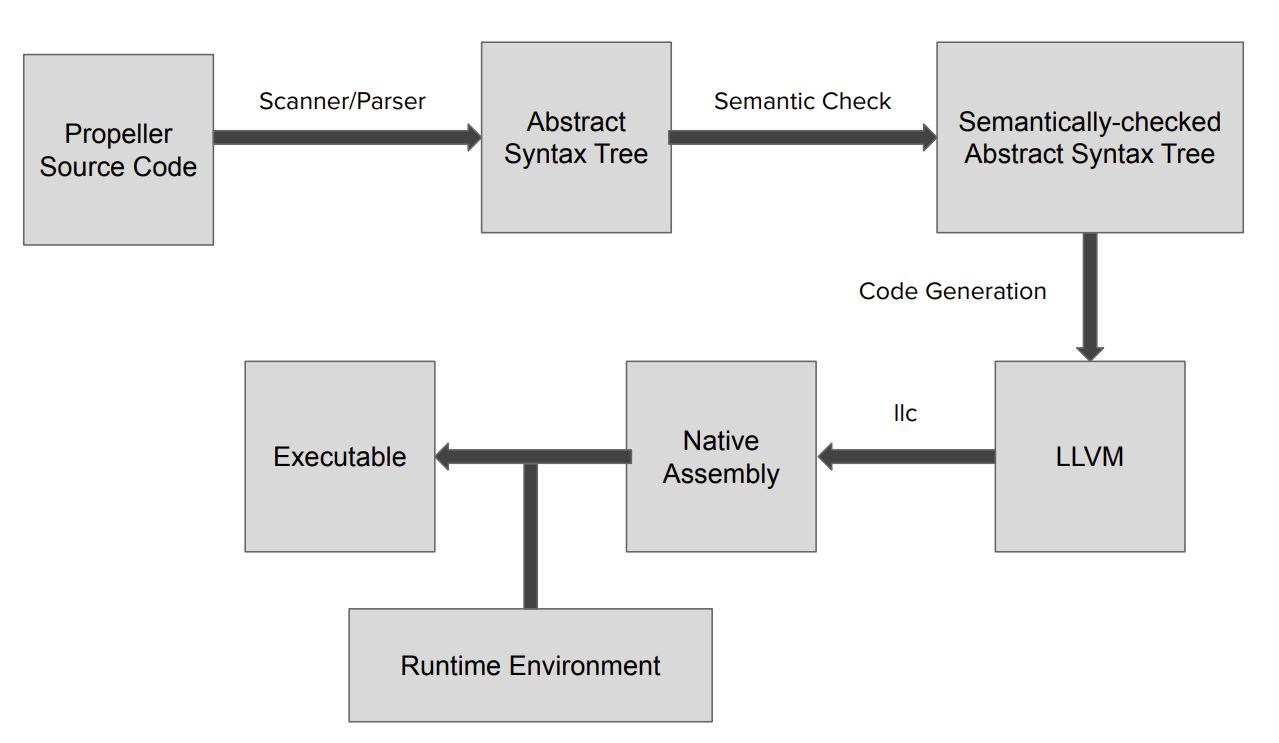
\includegraphics[scale=0.5]{block.jpg}
\end{center}

% Scanner
\subsection{Scanner}
The scanner transforms a Propeller program into a series of tokens, which are separated by
whitespace in the source code. Examples of tokens include variable names, function names,
types, separators, operators, control flow statements, and literals. Additionally, the
scanner throws a unique error if it encounters an ill-formed identifier (e.g.
\texttt{h?3\_\_llo}).

% Parser
\subsection{Parser}
The parser receives a series of tokens from the scanner, then uses these tokens to construct
an abstract syntax tree. Nothing of particular interest happens during the generation
of a Propeller program's AST.

% Semantic check
\subsection{Semantic Checker}
The semantic checker receives the AST from the parser, then performs various checks
on declarations, definitions, expressions, and statements. It prevents the programmer from
defining two or more functions with the same identifier, defining two or more
variables in the same scope with the same identifier, defining two or more object
types with the same identifier, overwriting a built-in function's definition,
using undefined identifiers, using undefined object properties, attempting to
access a property of a non-object variable, binding a function to a property
whose type does not match those of the function's formal parameters, binding a
function with some \texttt{n != 2} formal parameters to an object's property,
binding/unbinding a function to non-object variables, declaring variables of type
\texttt{void}, creating list literals of a non-primitive type, creating list
literals whose elements are of different types, passing an incorrect number of
arguments to a function, passing one or more arguments to a function whose types
does not match those of the function's formal parameters, returning a value whose
type does not match the function's return type, assigning a value to a variable
whose type differs from the value's type, and using unary and binary operators on
expressions with inappropriate types, and using \texttt{continue} or
\texttt{break} statements outside of loops. Once these checks are performed, the
semantic checker generates a semantically-checked abstract syntax tree.

% Code Generator
\subsection{Code Generator}
The code generator receives the SAST from the semantic checker, then converts
the SAST into an LLVM IR of the original Propeller program. Several additional
checks are performed as the instructions are being generated, which prevent
duplicate bindings of a function to the same property, prevent the unbinding
of a function from a property if it is not already bound, and assignment of
properties to external objects. 

\subsubsection{Bindings}
Bindings are processed in the code generation phase. It
keeps track of which functions are bound to the properties of object
variables using a single string map, which maps a combination of object
variable names and their properties to a list of function names.

% Runtime Environment
\subsection{External objects and Runtime Environment}
External objects are treated uniquely by Propeller. They are
not objects that occupy memory spaces in the Propeller module; instead, all
Propeller code treats them as integer values, like an identification for the
corresponding instance.

The sole purpose of runtime environments in Propeller is to provide
implementation of external objects. All interactions with external objects
within propeller are translated into calls to functions in the runtime
environment.

For each external object type, the runtime environment must implement\\
\verb|int object_new_<typename>()|, which creates an object of \verb|typename|
and returns its identification.

For each property of object type \verb|typename|, four functions must be
implemented:
\begin{itemize}
\item \verb|prop_t object_prop_get_<typename>_<propname>(int id)|: Gets the
value of property \verb|propname| of object with id \verb|id|. The return type
must match that of the property.
\item \verb|void object_prop_assign_<typename>_<propname>(int id, prop_t val)|:
Assign \verb|val| to the value of property \verb|propname| of object with id
\verb|id|. This is not actually implemented because we don't have a use for it
since GUI support is cancelled.
\item \verb|void object_prop_bind_<typename>_<propname>(int id, funcptr_t func)|:
Bind a function to the property \verb|propname| of object with id \verb|id|.
\verb|func| is a function in the Propeller module and is guaranteed to take two
parameters of the same type of the property.
\item \verb|void object_prop_unbind_<typename>_<propname>(int id, funcptr_t func)|:
Same as above, but unbinds the function.
\end{itemize}

Since Propeller does not have garbage collection capabilities yet, the runtime
cannot delete any of the objects it creates.

The runtime environment is required to run the entry point to the Propeller module
\verb|init()| on startup, then it can run any routine that's needed to notify the
Propeller module of changes of property values. They are usually implemented as
an ``event loop", either with polling or wait for some system calls to return.

% Work split
\subsection{Component-level work split}

\begin{itemize}
\item Lexer: Randy
\item Parser: Randy
\item Semantic Analysis:
  \begin{itemize}
  \item base SAST transformation: Randy
  \item function: Randy
  \item operators, expressions: Randy
  \item lists: Isra and Randy
  \item strings: Isra and Chris
  \item if statement: Randy
  \item while statement: Randy and Chris
  \item break and continue statement: Chris
  \item for statement: Randy
  \item return statement: Randy and Chris
  \item built-in functions: Randy and Isra
  \item objects: Randy
  \item external objects: Chris
  \item bindings: Randy
  \end{itemize}
\item Code generation:
  \begin{itemize}
    \item function: Randy
    \item return: Chris
    \item integer literals: Randy
    \item boolean literals and operators: Gwendolyn
    \item modulo operator: Chris
    \item float literals: Randy
    \item other binary and unary operators: Randy
    \item if statement: Randy
    \item while statement: Randy and Chris
    \item break and continue statement: Chris
    \item for statement: Randy
    \item list literals: Isra
    \item objects: Randy
    \item strings: Isra
    \item bindings: Randy
    \item external object bindings: Chris
    \item built-in functions: Randy, Isra and Chris
  \end{itemize}
\item Runtime: Chris
\end{itemize}

\section{Testing}

All testing facility is located in the \texttt{tests} directory of the compiler source code.

\subsection{Example source code and generated LLVM IR}

See Appendix B.

\subsection{Test scripts}

See Appendix C. Each function is documented in the comment above it.

\subsection{Test Automation}

A 105-style testing interface (notably the name ``CheckExpect") was used. The testing interface
as well as all test scripts are written in Bash. Three different aspects
of execution result can be checked against a given standard: standard output, standard error and
return code. The first two can be ignored if needed. Since the compiler exits with non zero return
code if an invalid program is fed to it, it can be used to verify test cases in which the
compilation is expected to fail.

There are convenience wrapper functions of \verb|CheckExpectWReturnCode| provided for different
tasks to simplify the process to make a test suite.

For each test suite, a test script is created. Running these test scripts will run all the tests
in that test suite.

\subsection{Testing task split}

The current testing framework is written by Chris. Parser unit tests are provided by Gwendolyn
and Isra. All team members contributed to the extended test suite. Previously the project used
a testing script written by Gwendolyn that was based on the test script of MicroC.

\section{Lessons learned} 

\subsection{Isra}

\subsection{Gwendolyn}

\subsection{Randy}
\begin{itemize}
    \item Functional programming is super cool, but it has its limits. We resorted to using a
          StringMap reference (which behaves like a global variable of sorts) to keep track of what
          functions are bound to the properties of object variables. I'm sure there's a
          functional way to do that, but this approach made the most sense to us.
    \item Start early, on everything! Code generation can get particularly hairy.
    \item The OCaml LLVM API can be pretty confusing, so be sure to ask your advisor a bunch
          of questions if you can't figure out how to get something working.
    \item Temper your expectations from the beginning. Your language should only have a handful of
          core features are unique and super exciting - don't promise too much!
\end{itemize}

\subsection{Chris}
\begin{itemize}
\item Even after been warned multiple times, I still have the habit of not starting the real work
until the last minute.
\item Functional programming is fun in a way that it forces me to think in completely different
patterns.
\item (As advice for future students as well) Learn to manage the expectations. As initially
planned, Propeller was clearly way too ambitious, even with GUIs, high-level list operations and
all the bells and whistles. As time flew by, some of the goals are clearly unrealistic for a
semester-long project and had to be dropped.
\item (When implementing external object bindings) If searching something gives no useful results,
and all hope is lost, trying all possible combinations could be a good way to go.
\item Test-oriented development can be beneficial, but could result in a compiler that doesn't work
with code that uses any untested features.
\item Function pointers in LLVM causes even more confusion than function pointers in C++.
\item I feel like as a team made of complete strangers, we could use more communication throughout
the project.
\end{itemize}

\section{Appendix A: Full Git Log}

{\scriptsize
\begin{verbatim}
commit 3545e6da4ba101248f0b5eab3e230309db5335f2
Author: Chris Xiong <chirs241097@gmail.com>
Date:   Sat May 7 21:49:48 2022 -0400

    Add final report.

commit 641256ceb066d25d952cba803350f2b88cd8abc2
Author: Chris Xiong <chirs241097@gmail.com>
Date:   Sat May 7 20:06:40 2022 -0400

    Update readme.

commit 80b3437c49f4eba727a9ca29efaff6bee8da5dfd
Author: Chris Xiong <chirs241097@gmail.com>
Date:   Sat May 7 20:03:59 2022 -0400

    Add author list to all OCaml source files.

commit fe849f5c2493275bad3a9bd18b715ca201f9e55d
Author: Chris Xiong <chirs241097@gmail.com>
Date:   Sat May 7 19:38:07 2022 -0400

    Update readme and description for new tests.

commit e27ca020f25e027f3f7b229c36a6844202a19cd9
Author: Chris Xiong <chirs241097@gmail.com>
Date:   Sat May 7 19:28:32 2022 -0400

    Add makefile and make targets for demo.

commit 857c7d8bc50aa8b9042a847150a7bf04fe3c761d
Author: Chris Xiong <chirs241097@gmail.com>
Date:   Sat May 7 19:20:43 2022 -0400

    Move demo code to its own directory.

commit 2920e1656ea29d9d3d0446c2599b8bf7f0cf01bf
Author: Chris Xiong <chirs241097@gmail.com>
Date:   Sat May 7 19:14:05 2022 -0400

    Fix all tests that doesn't work.

commit 714515ee6527d6ce47cf06fccfde6ef39bf35501
Author: Chris Xiong <chirs241097@gmail.com>
Date:   Sat May 7 18:35:20 2022 -0400

    Tidy up the demo code a bit.

commit caaef3ba6ff55dbf0084c3b788c76ef629bf2f9c
Author: Randy Price <edward.randolph.price@gmail.com>
Date:   Sat May 7 16:50:20 2022 -0400

    Add more detail to some error messages.

commit 2fdc64ab9041633c586c79339dfc6653cd91fddc
Author: Randy Price <edward.randolph.price@gmail.com>
Date:   Sat May 7 16:50:01 2022 -0400

    Add presentation slides.

commit 0adcdcf6bf15153b0dcc99d655d08479caa8f7b7
Author: Randy Price <edward.randolph.price@gmail.com>
Date:   Sat May 7 13:50:24 2022 -0400

    Refactor binding-related stuff in codegen.ml

commit 87a2018218c6f72a066fe4d571c7e3fdbb9db03e
Merge: 9543666 981fce2
Author: randyprice <79062334+randyprice@users.noreply.github.com>
Date:   Sat May 7 13:17:10 2022 -0400

    Merge branch 'main' of https://github.com/gfaline/Compilers

commit 954366669afebc0615fdbb3af5acd6516af920a0
Author: Randy Price <edward.randolph.price@gmail.com>
Date:   Sat May 7 13:17:04 2022 -0400

    Refactor SCall

commit bdb51b6c37ff410f3ad992a4a52bb2ec475ec330
Author: Randy Price <edward.randolph.price@gmail.com>
Date:   Sat May 7 13:07:47 2022 -0400

    List indexing works! Code cleanup to come.

commit 981fce2ae4a675615b5f9e4e36f01240e57a4d10
Author: Chris Xiong <chirs241097@gmail.com>
Date:   Sat May 7 12:41:49 2022 -0400

    Implement all interfaces in the sensor runtime.

commit 3e4be31de3db20d3a00a271367096862497283fe
Author: Chris Xiong <chirs241097@gmail.com>
Date:   Sat May 7 12:41:09 2022 -0400

    Update the sensor demo.

commit a43d90b632486556796f7ee20facb796b9bdfe42
Author: Chris Xiong <chirs241097@gmail.com>
Date:   Sat May 7 12:39:04 2022 -0400

    Fix prop get for external objects.
    
    Mark assignment to external objects as unimplemented.

commit 0a1a4f91bddd1112169058c1dbb4db867553277a
Author: Randy Price <edward.randolph.price@gmail.com>
Date:   Sat May 7 12:03:15 2022 -0400

    Remove redunant wildcard case in stmt.

commit 22bcc2c99c20056e4a117c06771e22608b5ce995
Author: Chris Xiong <chirs241097@gmail.com>
Date:   Sat May 7 11:09:59 2022 -0400

    Strip away the quotes and unescape special characters in strings.

commit de9e239b488ce0994640050b578e63877c8a2f84
Author: Chris Xiong <chirs241097@gmail.com>
Date:   Sat May 7 11:09:03 2022 -0400

    Whoopsie, got the parameters backwards.

commit 666ce2c013243fef61e3ebc7d74944fafcab824e
Author: ihamid01 <64386261+ihamid01@users.noreply.github.com>
Date:   Sat May 7 06:17:02 2022 -0400

    Rename propeller/tests/test-list.exp to propeller/tests/exttest/test-list.exp

commit 20a547bb1c6da5d60d09512cda3ca23f1ace7f87
Author: ihamid01 <64386261+ihamid01@users.noreply.github.com>
Date:   Sat May 7 06:16:39 2022 -0400

    Rename propeller/tests/test-list.pr to propeller/tests/exttest/test-list.pr

commit 437a86dab9db7d1401a61d8465a40deea9747de4
Author: ihamid01 <64386261+ihamid01@users.noreply.github.com>
Date:   Sat May 7 06:16:01 2022 -0400

    Create test-list.exp

commit b28f1fa7326b944826372a4a27b2488462845fff
Author: ihamid01 <64386261+ihamid01@users.noreply.github.com>
Date:   Sat May 7 06:15:19 2022 -0400

    Create test-list.pr

commit 221ccc4591a55631ecd1f90a39f322428803c698
Author: ihamid01 <64386261+ihamid01@users.noreply.github.com>
Date:   Fri May 6 08:23:57 2022 -0400

    Create test-print.exp

commit 5a67ca20c5841ce77c7fb87cdfdf063340523137
Author: ihamid01 <64386261+ihamid01@users.noreply.github.com>
Date:   Fri May 6 08:23:24 2022 -0400

    Create test-print.pr

commit 85f59e9a1769f3eda32ff384af8ce24f27658350
Merge: c6f30eb aa9eaf7
Author: randyprice <79062334+randyprice@users.noreply.github.com>
Date:   Fri May 6 08:21:50 2022 -0400

    Merge branch 'main' of https://github.com/gfaline/Compilers

commit aa9eaf7d5ca1a03fd63e71b600623e647ec283dd
Author: ihamid01 <64386261+ihamid01@users.noreply.github.com>
Date:   Fri May 6 08:21:40 2022 -0400

    Added print functions

commit c6f30eb91d44c7dd0501db5f0da4cdb3b4df5844
Author: Randy Price <edward.randolph.price@gmail.com>
Date:   Fri May 6 08:21:32 2022 -0400

    add silly demos

commit 78c13d76604df4254a2fc27fc0397bf9546462cf
Author: ihamid01 <64386261+ihamid01@users.noreply.github.com>
Date:   Fri May 6 08:19:24 2022 -0400

    List and print functions

commit cebe078a99a169c538cc144c6a07585c1cd78f24
Author: Chris Xiong <chirs241097@gmail.com>
Date:   Fri May 6 02:27:53 2022 -0400

    Implement external objects. Fix LLVM error that occurs if a function has no return value.
    
    Added sensor demo.
    Added the runtime system.
    Renamed entry point (main -> init).
    Updated tests to reflect these changes.

commit dc841cddc99f0c79f85364a1de0f28be5913b12d
Merge: 107e6cc 73255a0
Author: randyprice <79062334+randyprice@users.noreply.github.com>
Date:   Thu May 5 18:43:45 2022 -0400

    Merge branch 'main' of https://github.com/gfaline/Compilers

commit 107e6ccf9c824298f7596a74984e094e1a69b9bf
Author: Randy Price <edward.randolph.price@gmail.com>
Date:   Thu May 5 18:41:29 2022 -0400

    Add silly but kind of functional implementation of bind/unbind.

commit 73255a0000559cab54851f7cf20b66b32950c7dd
Author: ihamid01 <64386261+ihamid01@users.noreply.github.com>
Date:   Thu May 5 04:25:25 2022 -0400

    Updates SSliteral, scall print, and index
    
    Printing values other than integers causes an argtype error. Index is close to working but it's returning incorrect values.

commit 8141e617beb70f611988a336b98786b0be03e212
Author: ihamid01 <64386261+ihamid01@users.noreply.github.com>
Date:   Thu May 5 01:39:37 2022 -0400

    Update codegen.ml

commit 65a5188bc53fd6e18430b10192ab2b03c8567940
Author: ihamid01 <64386261+ihamid01@users.noreply.github.com>
Date:   Thu May 5 01:34:13 2022 -0400

    Update codegen.ml

commit 58dab46f1c20b7d5d29936008db76e3c5847849d
Author: ihamid01 <64386261+ihamid01@users.noreply.github.com>
Date:   Wed May 4 07:12:50 2022 -0400

    Update codegen.ml

commit 5634822440ecb5cff7e3ab11547ac213982eca3d
Author: Randy Price <edward.randolph.price@gmail.com>
Date:   Tue May 3 23:09:14 2022 -0400

    Add semantic check to bind.

commit c161dc4c720eb73e5263ea59da8a19145e61bb74
Author: Randy Price <edward.randolph.price@gmail.com>
Date:   Tue May 3 22:08:41 2022 -0400

    Add objects to codegen.ml - currently just act as structs.

commit 810646781d9e8d4960d4909a3af7c8229c74aedb
Author: Randy Price <edward.randolph.price@gmail.com>
Date:   Mon May 2 20:21:40 2022 -0400

    Comment out other list-related code in codegen.ml.

commit d911f9e2cf5a04f647b443694d01f8cb7530dbf9
Author: Randy Price <edward.randolph.price@gmail.com>
Date:   Mon May 2 20:19:56 2022 -0400

    Comment out incompelte code for lists in codegen.ml.

commit 7e41f9263c910b6a1e261cd5d39e51ef9ecbdec2
Author: Randy Price <edward.randolph.price@gmail.com>
Date:   Mon May 2 20:18:29 2022 -0400

    Fix missing opening comment symbol (* in codegen.ml.

commit edef96fe9aa8e8d31ee303c05dffb6d1cb520eca
Author: ihamid01 <64386261+ihamid01@users.noreply.github.com>
Date:   Sat Apr 30 21:10:42 2022 -0400

    Update codegen.ml

commit 8592dbbbc083bff7deb73cdd0e86442f23091fc2
Author: ihamid01 <64386261+ihamid01@users.noreply.github.com>
Date:   Sun Apr 24 08:02:06 2022 -0400

    Update codegen.ml

commit 96fe5afeec7b4e5b0b5f2d151e66503f93353c97
Author: ihamid01 <64386261+ihamid01@users.noreply.github.com>
Date:   Sun Apr 24 07:51:14 2022 -0400

    Update codegen.ml

commit babb96e85aaf32241f3894fcf0efdda5323b49ed
Author: Chris Xiong <chirs241097@gmail.com>
Date:   Wed Apr 20 15:42:14 2022 -0400

    Prepare archive for submission.

commit 249aceed98b7512e700df99def811c63098ad37a
Author: Chris Xiong <chirs241097@gmail.com>
Date:   Wed Apr 20 02:28:07 2022 -0400

    Update readme for the "Extended Testsuite" deliverable.

commit 7c9befa4062b8f0d30e6cedc171df10b663753af
Author: Chris Xiong <chirs241097@gmail.com>
Date:   Wed Apr 20 02:11:33 2022 -0400

    Update expected output for parser tests due to changes in the ast printer.

commit 0870b66adca9a2d731b35538f7d23bb0a7c84e4e
Author: Chris Xiong <chirs241097@gmail.com>
Date:   Wed Apr 20 02:00:55 2022 -0400

    Update the test target.

commit 39e0dc5a925606c754ccd3c0a1b310360e572db2
Author: Chris Xiong <chirs241097@gmail.com>
Date:   Wed Apr 20 01:59:05 2022 -0400

    One new test and a bunch of fixed descriptions.

commit 1974001a62492a7450e7d0fe67ce04660a3117b1
Author: Chris Xiong <chirs241097@gmail.com>
Date:   Wed Apr 20 01:41:00 2022 -0400

    Fix codegen for for-loops.

commit bb318140f18ef01f2cc04465eac008e0421388d0
Author: Chris Xiong <chirs241097@gmail.com>
Date:   Wed Apr 20 01:40:30 2022 -0400

    Even more tests (continue, for, function call).

commit 3119a0f0654f41613ef72eb25be1e3aa72e4ac7a
Merge: a6ef87d 5046568
Author: Randy Price <edward.randolph.price@gmail.com>
Date:   Wed Apr 20 01:11:05 2022 -0400

    Merge Chris's codegen with Randy's.

commit a6ef87d4758071199ab3da99056e288282dc3d6d
Author: Randy Price <edward.randolph.price@gmail.com>
Date:   Wed Apr 20 01:09:26 2022 -0400

    Add for loops to codegen.ml; nested for loops do not work.

commit 50465682ec78ef07885f27476e3cf24e0e546c3f
Author: Chris Xiong <chirs241097@gmail.com>
Date:   Wed Apr 20 00:50:04 2022 -0400

    Add tests for while, break and continue.

commit e5019493e1644337d9c41b298bb2443022fd723d
Author: Chris Xiong <chirs241097@gmail.com>
Date:   Wed Apr 20 00:49:08 2022 -0400

    Fix up codegen for while & implement break and continue.

commit 8cb0abe2664f558300fcf217f387a3c3e9412c32
Author: Chris Xiong <chirs241097@gmail.com>
Date:   Wed Apr 20 00:48:03 2022 -0400

    Improved diagnostics from the test script.

commit 04b1534125b762a4c025dd10e40f93cc28a232f3
Author: Randy Price <edward.randolph.price@gmail.com>
Date:   Wed Apr 20 00:13:43 2022 -0400

    Add looping variables as locals in semant.ml.

commit 5b36bf16346874225049e82edf97f15603d16000
Author: Chris Xiong <chirs241097@gmail.com>
Date:   Tue Apr 19 23:28:33 2022 -0400

    Add semantic check for break and continue and a relevant test.

commit f7ed39d6a94930b30faa461a2f948891d5d2f8be
Author: Chris Xiong <chirs241097@gmail.com>
Date:   Tue Apr 19 23:02:14 2022 -0400

    Add expected output for new tests and extended tests target in Makefile.

commit 9c7f81571a304933e873701a04e44d3a865dd2de
Author: Chris Xiong <chirs241097@gmail.com>
Date:   Tue Apr 19 22:57:11 2022 -0400

    Merge the two testsuites (expected output not ready yet).

commit 9d453f4eca797f845a2fc407996c32c2c85c7bb2
Author: Chris Xiong <chirs241097@gmail.com>
Date:   Tue Apr 19 22:48:28 2022 -0400

    Implement codegen for the modulo operator. Add tests.

commit bb8b8a7e3b74edab8fb6f6e3df8d7ca9d3f40af1
Author: gfaline <gwenfedgar@gmail.com>
Date:   Tue Apr 19 22:28:17 2022 -0400

    Two more tests, while isnt ready yet

commit 9b1b44f446b506663e57749c01f18ab4922de597
Merge: 41e824a a230e00
Author: gfaline <gwenfedgar@gmail.com>
Date:   Tue Apr 19 22:07:59 2022 -0400

    Merge branch 'main' of https://github.com/gfaline/Compilers

commit 41e824aaa0de8f1ef6bef802b7e15d8752f50bea
Author: gfaline <gwenfedgar@gmail.com>
Date:   Tue Apr 19 22:07:48 2022 -0400

    else test

commit a230e00a34d99b7a247849ec64990d6db3fa8ecb
Author: Chris Xiong <chirs241097@gmail.com>
Date:   Tue Apr 19 21:56:13 2022 -0400

    Make the compiler wrapper script fail cleanly.

commit 233f319411d42351b2fadc2a4cab7e738c6798f1
Author: gfaline <gwenfedgar@gmail.com>
Date:   Tue Apr 19 21:54:21 2022 -0400

    if elif else code, not testing yet

commit 3189f8a88bf93e5b638c35f0ff699b94c8678353
Author: Chris Xiong <chirs241097@gmail.com>
Date:   Tue Apr 19 21:31:49 2022 -0400

    Implement type checking on return statements.

commit ce0838e98fea490ff3b079dfc1e272afdbab70ea
Author: Chris Xiong <chirs241097@gmail.com>
Date:   Tue Apr 19 21:04:33 2022 -0400

    Eliminate all current warnings.

commit cad443c75731746d1e0af3381daaf436f7330b65
Author: Randy Price <edward.randolph.price@gmail.com>
Date:   Tue Apr 19 16:41:52 2022 -0400

    Add if/elif/else to codegen.ml.

commit e1d11171da188cb351d50a09fdcf31a8b9a06983
Author: Randy Price <edward.randolph.price@gmail.com>
Date:   Tue Apr 19 12:11:10 2022 -0400

    Add simple elif-less and else-less statements to codegen.ml.

commit b4e000e841e5896b9906ed70349beea9571f9f9a
Author: Randy Price <edward.randolph.price@gmail.com>
Date:   Tue Apr 19 11:43:31 2022 -0400

    Remove commented-out code. Rename local function in SWhile stmt case.

commit 888cc5d9c887ac170d0889112c45d6ca23db5759
Author: Randy Price <edward.randolph.price@gmail.com>
Date:   Tue Apr 19 11:41:24 2022 -0400

    Add while loops to codegen.ml.

commit e04be72acc52f859175023b59b7e06b863e93357
Author: Randy Price <edward.randolph.price@gmail.com>
Date:   Tue Apr 19 11:15:38 2022 -0400

    Minor typographical changes to ast.ml and sast.ml for consistency.

commit b978550af08c785850c672292c45364f87ee3189
Author: Randy Price <edward.randolph.price@gmail.com>
Date:   Tue Apr 19 11:14:24 2022 -0400

    Add simple function calls to codegen.ml.

commit cd8d1506f9d05d1830d993d594b8a398c4bed1be
Author: Randy Price <edward.randolph.price@gmail.com>
Date:   Tue Apr 19 11:00:33 2022 -0400

    Add noexpr to codegen.ml.

commit 324b3b921410fb002e729d170d3784e15af15819
Author: Randy Price <edward.randolph.price@gmail.com>
Date:   Tue Apr 19 10:58:52 2022 -0400

    Add simple id evaluation to codegen.ml.

commit 71db814eed672a627e547bffb8080383dcf107c2
Author: Randy Price <edward.randolph.price@gmail.com>
Date:   Tue Apr 19 10:54:54 2022 -0400

    Add simple variable assignment to codegen.ml.

commit b28f316c6d7cd35d8c410e14d3d2ae5813685452
Author: Randy Price <edward.randolph.price@gmail.com>
Date:   Tue Apr 19 10:46:10 2022 -0400

    Simplify printing of bool literals in sast.ml.

commit 2524d58b3c86aec46d73125bd96f2de645a70485
Author: Randy Price <edward.randolph.price@gmail.com>
Date:   Tue Apr 19 10:45:42 2022 -0400

    Simplify printing of bool literals in ast.ml.

commit 5aa2014c52c8ac76565022de08da6f34d0d99bf2
Author: Randy Price <edward.randolph.price@gmail.com>
Date:   Tue Apr 19 10:43:34 2022 -0400

    Add parentheses expr to codegen.ml.

commit 8dcc243e2825d44b92575e88c31cdddbf7b18da8
Author: Randy Price <edward.randolph.price@gmail.com>
Date:   Tue Apr 19 10:41:16 2022 -0400

    Add simply unary operators for ints, float, and bools to codegen.ml.

commit d97488a9a483b97ebe72f8be2086768ce7bcc62f
Author: Randy Price <edward.randolph.price@gmail.com>
Date:   Tue Apr 19 10:34:06 2022 -0400

    Add simple binary operators for int/float to codegen.ml.

commit 4923f3740b43a64642eb964ee7acfaa76361ec9b
Author: Randy Price <edward.randolph.price@gmail.com>
Date:   Tue Apr 19 10:12:41 2022 -0400

    Whoops, boolean literals were already there.

commit fa0ed40eb853b3cf0b2aa841f68a4af123a6f400
Author: Randy Price <edward.randolph.price@gmail.com>
Date:   Tue Apr 19 10:10:06 2022 -0400

    Add boolean literals to codegen.ml.

commit 6fc874ef58245e7519c18ad80ea5b395476245c9
Author: Randy Price <edward.randolph.price@gmail.com>
Date:   Tue Apr 19 10:02:53 2022 -0400

    Add global variables to codegen.ml

commit 680ab71ed671dea9457899a4e0cf5df81d8dc4b5
Author: Randy Price <edward.randolph.price@gmail.com>
Date:   Tue Apr 19 09:55:52 2022 -0400

    Add simple unbind to sast.ml and semant.ml.

commit d949d5f38ec61e4b8f252e0adec8282e6221badb
Author: Randy Price <edward.randolph.price@gmail.com>
Date:   Tue Apr 19 09:50:13 2022 -0400

    Add simple bind to sast.ml and semant.ml.

commit 9c458132dd8f9a655a29164e86103fbc0ab018ab
Merge: 57ce7b8 b503f1b
Author: Randy Price <edward.randolph.price@gmail.com>
Date:   Mon Apr 18 22:23:51 2022 -0400

    Merge codegen.ml with remote.

commit 57ce7b83dd948d95ad223c293361c160d89bb5e7
Author: Randy Price <edward.randolph.price@gmail.com>
Date:   Mon Apr 18 22:19:38 2022 -0400

    Add object property assignment to sast.ml and semant.ml.

commit 830e76616119e2a65246b14ce26e383023f275f1
Author: Randy Price <edward.randolph.price@gmail.com>
Date:   Mon Apr 18 22:09:13 2022 -0400

    Add object property dereferencing.

commit ddfb4eea621b2672e3acd3b2e13d82b4553e9921
Author: Randy Price <edward.randolph.price@gmail.com>
Date:   Mon Apr 18 19:54:24 2022 -0400

    Add comments to semant.ml.

commit 5c73a7fc4519dfcc363d544ed0db968eed133e5f
Author: Randy Price <edward.randolph.price@gmail.com>
Date:   Mon Apr 18 19:52:40 2022 -0400

    Simplify semant.ml.

commit 93485961f5bc9d810e90d79d24bb8deab06966f3
Author: Randy Price <edward.randolph.price@gmail.com>
Date:   Mon Apr 18 19:50:17 2022 -0400

    Add object definition to sast.ml and semant.ml. Simplify some printing things in the AST/SAST.

commit 45595c63d7ddcb3c536202a8176df88c4665b3e5
Author: Randy Price <edward.randolph.price@gmail.com>
Date:   Mon Apr 18 19:03:26 2022 -0400

    Add list indexing to sast.ml and semant.ml.

commit 9da4518dc94bc014a9ce2e6c4eabecfc0036aa6e
Author: Randy Price <edward.randolph.price@gmail.com>
Date:   Mon Apr 18 18:36:54 2022 -0400

    Add lists to sast.ml and semant.ml.

commit 798274a7fff99cf7295aae9142ff701950c697f0
Author: Randy Price <edward.randolph.price@gmail.com>
Date:   Mon Apr 18 17:37:20 2022 -0400

    Change OCaml representation of Propeller lists from list to array.

commit 526a245c23d59f36cd4df12c1c43fc293ca13262
Author: Randy Price <edward.randolph.price@gmail.com>
Date:   Mon Apr 18 16:57:41 2022 -0400

    Add break and continue to sast.ml and semant.ml.

commit 6675ae7e9475e5c5b3e19643eba8785da020ab43
Author: Randy Price <edward.randolph.price@gmail.com>
Date:   Mon Apr 18 16:52:49 2022 -0400

    Add simple while loops to sast and semant.ml.

commit 07815d38048ee19ab5125d4b90815084141a0f25
Author: Randy Price <edward.randolph.price@gmail.com>
Date:   Mon Apr 18 16:46:02 2022 -0400

    Add simple for loop to sast.ml and semant.ml.

commit e0dc68a4d1852dc2f678e2a43c61326ed7c66537
Author: Randy Price <edward.randolph.price@gmail.com>
Date:   Mon Apr 18 15:28:01 2022 -0400

    Add variable assignment to sast.ml and semant.ml.

commit 39ab29dd570edc5a7d01702b83822d625f054db0
Author: Randy Price <edward.randolph.price@gmail.com>
Date:   Mon Apr 18 15:22:06 2022 -0400

    Add ID evaluation to sast.ml and semant.ml.

commit 2d9edc7a6bdfe03e67749ecf10d3d13bcef54b5a
Author: Randy Price <edward.randolph.price@gmail.com>
Date:   Sun Apr 17 16:38:14 2022 -0400

    Fix typo in codegen.ml.

commit d5221d6ce9c82d16126972801f9e5dd1b3ea20f3
Author: Randy Price <edward.randolph.price@gmail.com>
Date:   Sun Apr 17 16:37:12 2022 -0400

    Add floats to codegen.ml.

commit a21f6de6234477b3487fd367c00608d55063a6ae
Author: Randy Price <edward.randolph.price@gmail.com>
Date:   Thu Apr 14 23:30:17 2022 -0400

    Add return to sast and semant.

commit e0ebcb7ca5a306999a1145ac12dfde56fa406ae1
Author: Randy Price <edward.randolph.price@gmail.com>
Date:   Thu Apr 14 23:21:02 2022 -0400

    Add full if/elif/else support to sast.ml and semant.ml.

commit 23248059d8848643fbf5766293ef2eab96ad202a
Author: Randy Price <edward.randolph.price@gmail.com>
Date:   Thu Apr 14 23:05:58 2022 -0400

    Apply code-reduction from ast.ml to sast.ml.

commit db52984db47fe6418e4d0fa5d8121d1f01ae5a5a
Author: Randy Price <edward.randolph.price@gmail.com>
Date:   Thu Apr 14 22:51:57 2022 -0400

    Add function brace_wrap to reduce code in ast.ml.

commit 403d642f5a30dd4a3aab9f167f842a9dea362550
Author: Randy Price <edward.randolph.price@gmail.com>
Date:   Thu Apr 14 22:28:54 2022 -0400

    Simplify string_of_stmt_list If case.

commit be82bedc044b684be38fe2aeb62c8d630452002b
Author: Randy Price <edward.randolph.price@gmail.com>
Date:   Thu Apr 14 21:58:05 2022 -0400

    Add else-less if-elif stmts to semant.ml.

commit 4f67597b9580408f4c284659f8f1321a65d277dd
Author: Randy Price <edward.randolph.price@gmail.com>
Date:   Thu Apr 14 21:28:15 2022 -0400

    Add elif-less if-else stmts to sast.ml and semant.ml.

commit 84c5eaf63630de2105b2e187de7679b3e432978c
Author: Randy Price <edward.randolph.price@gmail.com>
Date:   Thu Apr 14 21:23:27 2022 -0400

    Fix printing for elif-less if-else stmt in ast.ml.

commit d5fdf7dc0860c9d47b585aed58aee56eeaf63f11
Author: Randy Price <edward.randolph.price@gmail.com>
Date:   Thu Apr 14 21:20:09 2022 -0400

    Add elif-less and else-less if to sast.ml and semant.ml.

commit b152fb3d1720b76e38c72eac907510cd71c6779a
Author: Randy Price <edward.randolph.price@gmail.com>
Date:   Sat Apr 9 17:18:19 2022 -0400

    Add parentheses expression to sast.ml and semant.ml.

commit 6b85cc0134b33d426e8351902bccee01537e003e
Author: Randy Price <edward.randolph.price@gmail.com>
Date:   Sat Apr 9 17:04:19 2022 -0400

    Add unary operators to sast.ml and semant.ml.

commit b503f1bd8dd850535e561eddf6a532e9a12295cf
Author: gfaline <gwenfedgar@gmail.com>
Date:   Sat Apr 9 13:45:37 2022 -0400

    typo... now all compiling

commit 31da9ae0967302de94f2b51d0f27335878a1032d
Author: gfaline <gwenfedgar@gmail.com>
Date:   Sat Apr 9 12:47:05 2022 -0400

    minor fix, sorry

commit f5e75fc94f71302427f2d21dccbc1457e5c09fe1
Author: gfaline <gwenfedgar@gmail.com>
Date:   Sat Apr 9 11:44:41 2022 -0400

    Added boolean operators and stuff

commit 8959fe64aaa6848c29ee69934ec6f9b72410fedd
Author: Randy Price <edward.randolph.price@gmail.com>
Date:   Mon Apr 4 20:06:52 2022 -0400

    Add binary operators to sast.ml and semant.ml.

commit 93f670ca9e6c927203cfd610fd252e878ecc8682
Author: Randy Price <edward.randolph.price@gmail.com>
Date:   Sun Mar 27 18:55:20 2022 -0400

    Move README.md to propeller folder since it's often zipped with other files.

commit 3724244bebe93ff10c2d1249bb724fa9e562233b
Author: Randy Price <edward.randolph.price@gmail.com>
Date:   Sun Mar 27 18:54:13 2022 -0400

    Add submissions folder to keep track of past submissions. Initial commit contains hello-world.zip.

commit eddf52b52774b2fbc72f4463944112330cf7b677
Author: Randy Price <edward.randolph.price@gmail.com>
Date:   Sun Mar 27 18:45:35 2022 -0400

    Add .exe and .out to .gitignore.

commit b084d142658b0c39cd0bc5260383b04a4d56c0e5
Author: Randy Price <edward.randolph.price@gmail.com>
Date:   Sun Mar 27 18:44:23 2022 -0400

    Fix compilation issue by using more verbose useage of ocamlbuild from the MicroC README.

commit c754ff57abd30e147c8f597cc2267269d9a70821
Author: Randy Price <edward.randolph.price@gmail.com>
Date:   Sun Mar 27 18:43:10 2022 -0400

    Add comment to README regarding description of tests in source files.

commit 764fc148226ade1dc65894af9b111677608aab0a
Author: Randy Price <edward.randolph.price@gmail.com>
Date:   Sun Mar 27 18:41:43 2022 -0400

    Add comments to each source file that describe the nature of the feature it tests.

commit 9a0584eed413f879cbaf2b748dc522f05959a0b7
Author: Chris Xiong <chirs241097@gmail.com>
Date:   Fri Mar 25 13:31:30 2022 -0400

    Fix line endings for shell scripts.

commit 184ef20d369b2923a45723a4905338fa4df46eb3
Author: Chris Xiong <chirs241097@gmail.com>
Date:   Fri Mar 25 13:24:30 2022 -0400

    Try fixing some EOL shenanigans.

commit 1822c9d90db74b6c83f4113c404895b98c0bdfe3
Author: Randy Price <edward.randolph.price@gmail.com>
Date:   Fri Mar 25 13:10:51 2022 -0400

    Fix an eggregious butchering of Gwen's name by Randy.

commit bb6ccda34ddf5a3aeda2aedf25933ec4c969e4d5
Author: Chris Xiong <chirs241097@gmail.com>
Date:   Fri Mar 25 00:26:45 2022 -0400

    Update readme to reflect new testing infrastructure.

commit 737e734472442a02ebb4de0fc67c799f3d565ce7
Author: Chris Xiong <chirs241097@gmail.com>
Date:   Fri Mar 25 00:26:31 2022 -0400

    Add option for preserving intermediate files.

commit e8a22f3d9af0f9b9ab35e887de1958b13a2d4243
Author: Chris Xiong <chirs241097@gmail.com>
Date:   Fri Mar 25 00:26:07 2022 -0400

    Add a failure case for hello world tests.

commit eb370aab05cb6be84b0ffef7d71651693cde837f
Author: Chris Xiong <chirs241097@gmail.com>
Date:   Thu Mar 24 23:56:11 2022 -0400

    Update Readme.

commit 73bdc5d2303305e36196347a922d3c6da11e6bb1
Author: Chris Xiong <chirs241097@gmail.com>
Date:   Thu Mar 24 23:37:37 2022 -0400

    Add tests for hello world program. Add test targets to Makefile.

commit 650153a492550d3ac37d3c2f26b105faa4622c4a
Author: Chris Xiong <chirs241097@gmail.com>
Date:   Thu Mar 24 23:17:21 2022 -0400

    Remove duplicate leftover files from old testing scripts.

commit 9dd4ed4a755c79ef3a988fa393ba2b28b74578a6
Author: Chris Xiong <chirs241097@gmail.com>
Date:   Thu Mar 24 23:15:58 2022 -0400

    Rewritten the testing infrastructure.

commit ae47b5ad1a2be07a3e79e4fa5367e0b44db517c1
Author: Chris Xiong <chirs241097@gmail.com>
Date:   Thu Mar 24 20:10:45 2022 -0400

    Add bare bones implementation of return. Fix print and integer literals.

commit c9637cdb6b08d19781ca5c465e65e761c7341d07
Author: Chris Xiong <chirs241097@gmail.com>
Date:   Thu Mar 24 19:52:22 2022 -0400

    Eliminate all current warnings.

commit a342a28153c502978ebf94cbc58669ef85afcbc9
Author: Chris Xiong <chirs241097@gmail.com>
Date:   Thu Mar 24 19:34:30 2022 -0400

    Add basic makefile for the compiler.

commit 4b5feb4e5f2091826c03bd18455aa7f59c6a82be
Author: Chris Xiong <chirs241097@gmail.com>
Date:   Thu Mar 24 19:10:29 2022 -0400

    Ignore intermediate files in the compilation process.

commit 40e616955a06e97dde0f1a6007a05cf829b481a4
Author: Chris Xiong <chirs241097@gmail.com>
Date:   Thu Mar 24 19:08:24 2022 -0400

    Add wrapper script for complete compiling pipeline.

commit 86933f3b6c40c5ea5cefa6acd9ecb2fd193f2582
Author: Chris Xiong <chirs241097@gmail.com>
Date:   Thu Mar 24 18:35:02 2022 -0400

    Convert all files to LF line endings.
    
    ... and enforce LF on all text files in repository.

commit 3fba3a6e253a0910103beb11b447b2f9f70f47c5
Author: Randy Price <edward.randolph.price@gmail.com>
Date:   Thu Mar 24 17:01:43 2022 -0400

    Add str literals to sast.ml and semant.ml.

commit e2df34e84031560ccd42c2eed333488d9e277ad0
Author: Randy Price <edward.randolph.price@gmail.com>
Date:   Thu Mar 24 16:39:49 2022 -0400

    Add bool literals to sast.ml and semant.ml.

commit f957a997254eea5ee7cb63e0f0f7902f6517aff2
Author: Randy Price <edward.randolph.price@gmail.com>
Date:   Thu Mar 24 16:39:31 2022 -0400

    Add test.pr to gitignore.

commit 5226e9820cd747521a47e529cd69c3fcbccd8ef9
Author: Randy Price <edward.randolph.price@gmail.com>
Date:   Thu Mar 24 16:39:15 2022 -0400

    Remove test.pr (Randy's personal test file).

commit 28ca1d03a5701dffc6917cd5d391f5b8d81c875a
Author: Randy Price <edward.randolph.price@gmail.com>
Date:   Thu Mar 24 16:29:36 2022 -0400

    Fix bug in string_of_sexpr. Add float literals to sast.ml and semant.ml.

commit 708d430fbabd6996ea62a4f78e3733f7e3695cff
Author: Randy Price <edward.randolph.price@gmail.com>
Date:   Thu Mar 24 16:03:13 2022 -0400

    Fix context name.

commit b865448e04f8540608a8a3e5c67f09c1aacb1303
Author: Randy Price <edward.randolph.price@gmail.com>
Date:   Thu Mar 24 15:50:52 2022 -0400

    Simple 'hello world' program can now be compiled.

commit 740144ca7e50f7b33364a576f310bbcc7098e772
Author: Randy Price <edward.randolph.price@gmail.com>
Date:   Thu Mar 24 13:11:42 2022 -0400

    Add minimal codegen capabilities. LLVM IR can be printed.

commit 8acf2278dccfcf8d3b5efd43bd903fefda824ee1
Author: Randy Price <edward.randolph.price@gmail.com>
Date:   Wed Mar 23 20:30:37 2022 -0400

    Add empty codegen.ml, sast.ml, semant.ml.

commit e45bc5ebe94b6af112fcc125e04fd9383fd5996b
Author: Randy Price <edward.randolph.price@gmail.com>
Date:   Wed Mar 23 20:27:42 2022 -0400

    Rename scanner-parser folder to propeller.

commit 014eee06fef6b1e0f27247fac0a05068419db066
Author: Randy Price <edward.randolph.price@gmail.com>
Date:   Wed Mar 23 20:26:55 2022 -0400

    Add other lrm files.

commit 5b3b91066ce83fafb5cf154e8c6e7171b773f871
Merge: 77d2e94 3b7c2bc
Author: randyprice <79062334+randyprice@users.noreply.github.com>
Date:   Tue Mar 1 00:00:42 2022 -0500

    Merge branch 'main' of https://github.com/gfaline/Compilers

commit 3b7c2bc641fc4f45607145886e5a8730bb97c148
Author: Chris Xiong <chirs241097@gmail.com>
Date:   Mon Feb 28 23:55:22 2022 -0500

    Fix errors in tex files.

commit 77d2e94a3c34d472af2db992b36d04f8c06fee86
Author: randyprice <79062334+randyprice@users.noreply.github.com>
Date:   Mon Feb 28 23:57:19 2022 -0500

    Revert "Revert "Rewordings/corrections""
    
    This reverts commit de674e4116a3d7393d40c92afdeb81d1dc89421e.

commit de674e4116a3d7393d40c92afdeb81d1dc89421e
Author: randyprice <79062334+randyprice@users.noreply.github.com>
Date:   Mon Feb 28 23:52:50 2022 -0500

    Revert "Rewordings/corrections"
    
    This reverts commit 54035b5976cea53fe2dad2fb0f27e72ce3165367.

commit 5fc6651e947a4c4f1c234af5459a888f32c137b4
Author: Chris Xiong <chirs241097@gmail.com>
Date:   Mon Feb 28 23:52:41 2022 -0500

    crlf -> lf

commit 54035b5976cea53fe2dad2fb0f27e72ce3165367
Author: Randy Price <edward.randolph.price@gmail.com>
Date:   Mon Feb 28 23:48:30 2022 -0500

    Rewordings/corrections

commit 2daeefefd14c2523956f02d55e67c6a6addec5cb
Author: Chris Xiong <chirs241097@gmail.com>
Date:   Mon Feb 28 22:26:37 2022 -0500

    Manually merged with the LRM project on overleaf.

commit 51c421ec52533f594c90fec93fd0cff708251b79
Author: Chris Xiong <chirs241097@gmail.com>
Date:   Mon Feb 28 19:45:51 2022 -0500

    LRM updates for lists.

commit 79ec1a46a84d7427ee468e8d42e22ad387fc8407
Author: Chris Xiong <chirs241097@gmail.com>
Date:   Mon Feb 28 18:41:46 2022 -0500

    Update LRM to reflect the new identifier rule.

commit f30500038a77d03d0887eb5f759250c7a4f0b603
Author: Randy Price <edward.randolph.price@gmail.com>
Date:   Mon Feb 28 13:18:55 2022 -0500

    Removed commented-out code.

commit cf0ab4f5f3e2c1fb06c17118b154a6b32f081a69
Merge: 8be36ab edc0a5a
Author: randyprice <79062334+randyprice@users.noreply.github.com>
Date:   Mon Feb 28 13:17:04 2022 -0500

    Merge branch 'main' of https://github.com/gfaline/Compilers

commit 8be36ab703cf1e99289b8433483f974c19bc7831
Author: Randy Price <edward.randolph.price@gmail.com>
Date:   Mon Feb 28 13:16:29 2022 -0500

    Simplified regex for valid identifiers.

commit edc0a5afd4275b3aa7a75a9b0e5d6270cca2d52c
Author: randyprice <79062334+randyprice@users.noreply.github.com>
Date:   Sun Feb 27 16:17:27 2022 -0500

    Fix typo in scanner.

commit 7f582bc4ccc3c14ca5345ab71d4fb329e53331a0
Author: randyprice <79062334+randyprice@users.noreply.github.com>
Date:   Sun Feb 27 14:23:12 2022 -0500

    Add external keyword. Modify obj_decl to include extern field (bool).

commit 1f7b714f56b06aead33676c64c63512dea5425ad
Author: randyprice <79062334+randyprice@users.noreply.github.com>
Date:   Sun Feb 27 13:13:43 2022 -0500

    Add declaration of variables of custom types.

commit 1e7b5d1aff77ebf7f8a9b63888f2d497ad5fe979
Author: Chris Xiong <chirs241097@gmail.com>
Date:   Sun Feb 27 10:21:02 2022 -0500

    LRM initial edition.

commit 69fc853e513495d3fc78f4b5054108079a6889fa
Author: Randy Price <edward.randolph.price@gmail.com>
Date:   Fri Feb 25 11:39:13 2022 -0500

    Modified testall.sh to remove any CR from output files. Tests should now be platform-agnostic.

commit a0a2563874be651cf3ea61bbc1b303413f7bab9b
Author: Chris Xiong <chirs241097@gmail.com>
Date:   Fri Feb 25 10:37:53 2022 -0500

    purge useless files generated by macOS.

commit 59c65926e75112c44ecbc83765e62e0a7a21a427
Author: randyprice <79062334+randyprice@users.noreply.github.com>
Date:   Fri Feb 25 10:37:33 2022 -0500

    Delete test-*.ll.
    
    Seems to have been committed by mistake - it's preventing me from pulling.

commit c334a0ecf8bb4fa5f44495fb4841613881ce407e
Author: gfaline <gwenfedgar@gmail.com>
Date:   Thu Feb 24 21:04:31 2022 -0500

    5th fixed

commit fb5285424ebfad23759949746feff5ac83084e68
Author: gfaline <gwenfedgar@gmail.com>
Date:   Thu Feb 24 20:51:09 2022 -0500

    Update .gitignore
    
    Just another testing generated file

commit 1021870f388169eababe1c7ec83a529b9375c9aa
Author: gfaline <gwenfedgar@gmail.com>
Date:   Thu Feb 24 20:49:49 2022 -0500

    Update testall.sh
    
    Didnt go back enough commits. Manually fixed it.

commit f2f802887c3831a6560ae5d7be9b7512cf6219f6
Merge: d18fba7 c3da99a
Author: gfaline <gwenfedgar@gmail.com>
Date:   Thu Feb 24 20:48:50 2022 -0500

    Merge pull request #9 from gfaline/testing_fix
    
    Testing fix

commit d18fba756f397a277f26515966deefe80373b975
Author: gfaline <gwenfedgar@gmail.com>
Date:   Thu Feb 24 20:45:47 2022 -0500

    Revert "Update testall.sh"
    
    This reverts commit dd5d63f990732d83cab4f9d6b588b68dbcd364c4.

commit 2b90a9d7134316f3ee70eeb66468456a6c36c144
Author: gfaline <gwenfedgar@gmail.com>
Date:   Thu Feb 24 20:44:15 2022 -0500

    Fixing the deletion stuff....
    
    Revert "Added newline to end end of string_of_program."
    
    This reverts commit f66cac8acb0b4a41d550dc7174fdd3a147182c30.

commit c3da99a63b8f9b5f8ab420005f7e4f20b34e7e09
Author: gfaline <gwenfedgar@gmail.com>
Date:   Thu Feb 24 20:41:02 2022 -0500

    Testing fix

commit dd5d63f990732d83cab4f9d6b588b68dbcd364c4
Author: ihamid01 <64386261+ihamid01@users.noreply.github.com>
Date:   Thu Feb 24 18:23:51 2022 -0500

    Update testall.sh

commit 895452f7a90062004f6d8720d646289a6ae6eaf2
Author: ihamid01 <64386261+ihamid01@users.noreply.github.com>
Date:   Thu Feb 24 17:39:39 2022 -0500

    Update testall.sh

commit f66cac8acb0b4a41d550dc7174fdd3a147182c30
Author: Randy Price <edward.randolph.price@gmail.com>
Date:   Thu Feb 24 11:50:48 2022 -0500

    Added newline to end end of string_of_program.

commit bc2b3452165540124798c36e641fc35ffcf614b2
Author: Randy Price <edward.randolph.price@gmail.com>
Date:   Thu Feb 24 11:49:50 2022 -0500

    Removed runtests.py

commit e2b5ac6d43fa9c6a147b98592453cd87c8dcc72b
Author: gfaline <gwenfedgar@gmail.com>
Date:   Thu Feb 24 10:47:19 2022 -0500

    Tests

commit e3fb60db08ecb8384d9ab79a72ed311ac16b0e43
Author: gfaline <gwenfedgar@gmail.com>
Date:   Thu Feb 24 10:27:36 2022 -0500

    Added a requirements line

commit 75c00dd9801ed1dec18ec5f61c7e3740934787a8
Author: gfaline <gwenfedgar@gmail.com>
Date:   Thu Feb 24 10:26:25 2022 -0500

    Trying to do minor formatting.

commit f4ed1c68afe36afb93ec80252b4c464303220d34
Merge: 7db7f42 765974e
Author: gfaline <gwenfedgar@gmail.com>
Date:   Thu Feb 24 10:25:45 2022 -0500

    Merge pull request #7 from gfaline/testing
    
    Testing

commit 765974e9f302714ec42b7518d071d2cbffd1f780
Merge: ce7f6a6 7db7f42
Author: gfaline <gwenfedgar@gmail.com>
Date:   Thu Feb 24 10:25:30 2022 -0500

    Merge branch 'main' into testing

commit ce7f6a6cc3ea4904757f6e10b9670d7f453eadb1
Author: ihamid01 <64386261+ihamid01@users.noreply.github.com>
Date:   Thu Feb 24 03:11:06 2022 -0500

    Delete fail-test4.pr.diff

commit 77eceb3082257a31e01cecf29c149cc60003e032
Author: ihamid01 <64386261+ihamid01@users.noreply.github.com>
Date:   Thu Feb 24 03:10:56 2022 -0500

    Delete fail-test3.pr.diff

commit 7d50c4c14056f60d4f83cb59127e9767a04b4a72
Author: ihamid01 <64386261+ihamid01@users.noreply.github.com>
Date:   Thu Feb 24 03:10:43 2022 -0500

    Delete fail-test2.pr.diff

commit 806d1e708e16a2b1c1cfca8851b57a4c8e0868de
Author: ihamid01 <64386261+ihamid01@users.noreply.github.com>
Date:   Thu Feb 24 03:10:32 2022 -0500

    Delete fail-test1.pr.diff

commit 5bc4d1f136245d7d210be51bbe1fe7fe95e9f52b
Author: ihamid01 <64386261+ihamid01@users.noreply.github.com>
Date:   Thu Feb 24 03:10:20 2022 -0500

    Delete fail-test5.pr.diff

commit 7db7f42f7fa8ebf938f933b3aa698f5fc0b369c5
Author: ihamid01 <64386261+ihamid01@users.noreply.github.com>
Date:   Thu Feb 24 03:08:57 2022 -0500

    Delete fail-test1.pr.diff

commit 8a2e548582c151d2e9ad15e2f93af5638905826e
Author: ihamid01 <64386261+ihamid01@users.noreply.github.com>
Date:   Thu Feb 24 03:08:32 2022 -0500

    Add files via upload

commit 537d9e671771dc7628a3374fdeecd2dd4155e390
Author: ihamid01 <64386261+ihamid01@users.noreply.github.com>
Date:   Thu Feb 24 03:08:21 2022 -0500

    Add files via upload

commit ba49f4151b8cf2f9a9fb4edaa63e35d819460d94
Author: ihamid01 <64386261+ihamid01@users.noreply.github.com>
Date:   Thu Feb 24 03:07:40 2022 -0500

    Delete fail-test5.pr.diff

commit d36882e3ae0dd3cf384264b8d626774eedb8bd18
Author: ihamid01 <64386261+ihamid01@users.noreply.github.com>
Date:   Thu Feb 24 03:07:19 2022 -0500

    Delete fail-test4.pr.diff

commit 7d3e195c6a55659c35ce159eae5d48c348990401
Author: ihamid01 <64386261+ihamid01@users.noreply.github.com>
Date:   Thu Feb 24 03:07:11 2022 -0500

    Delete fail-test3.pr.diff

commit afea738ec41b7b658d4924cf0b9942e5847be308
Author: ihamid01 <64386261+ihamid01@users.noreply.github.com>
Date:   Thu Feb 24 03:06:53 2022 -0500

    Delete fail-test2.pr.diff

commit 949ded4929c4cef4c81f3e29f383488400c36b64
Author: ihamid01 <64386261+ihamid01@users.noreply.github.com>
Date:   Thu Feb 24 03:06:40 2022 -0500

    Delete fail-test1.pr.diff

commit 3210cc91325d1244126a989ddd9535448c1da352
Author: ihamid01 <64386261+ihamid01@users.noreply.github.com>
Date:   Thu Feb 24 03:05:20 2022 -0500

    Add files via upload

commit 5881a0138a26e2d3929de276babaacbb28a6073d
Author: Randy Price <edward.randolph.price@gmail.com>
Date:   Wed Feb 23 23:25:23 2022 -0500

    Added description of differences between MicroC and Propeller, saying to assume that simple things were lifted from MicroC unless otherwise noted.

commit 3bfa1c728079e10abf8ce8889934fc02503dc29d
Author: Randy Price <edward.randolph.price@gmail.com>
Date:   Wed Feb 23 22:29:17 2022 -0500

    Added document containing examples of Propeller syntax.

commit 88cb8e5ee7599775cba1f5a4474adb83297b3143
Author: Randy Price <edward.randolph.price@gmail.com>
Date:   Wed Feb 23 22:28:43 2022 -0500

    Changed syntax of bind/unbind. Functions are now bound to object properties, not objects themselves. Fixed an issue where an empty list local variables would result in a blank line being printed in string_of_fdecl.

commit 8ab9045a2357128fdb208e0c0c169f12ba66e36e
Author: Randy Price <edward.randolph.price@gmail.com>
Date:   Wed Feb 23 21:33:33 2022 -0500

    Organized expr rules, expr type definition, and string_of_expr.

commit 1402546c74ae5ed0a472205dfff6c18d172ea863
Author: Randy Price <edward.randolph.price@gmail.com>
Date:   Wed Feb 23 21:20:56 2022 -0500

    Added list indexing.

commit df9142f4fbbfa556c1fed43ed5f2486e719f88a9
Merge: 642531a 2f2a7d4
Author: gfaline <gwenfedgar@gmail.com>
Date:   Wed Feb 23 20:35:26 2022 -0500

    Master merge

commit 2f2a7d45ebdd07b2e77b75cb12d27852eeac2455
Author: gfaline <gwenfedgar@gmail.com>
Date:   Wed Feb 23 20:33:47 2022 -0500

    More generated files being exculded

commit 642531ab8e1bbb8372bc448061887a86db1b7a66
Author: gfaline <gwenfedgar@gmail.com>
Date:   Wed Feb 23 20:32:48 2022 -0500

    Readme change

commit 4aebc59715a6acde4636ecdb14f795118fa8f851
Author: gfaline <gwenfedgar@gmail.com>
Date:   Wed Feb 23 20:18:52 2022 -0500

    it runs! Gotta check that it should be passing,ool

commit 443f2dd0eb0a7e44ce9f08cc66e954953b482977
Author: gfaline <gwenfedgar@gmail.com>
Date:   Wed Feb 23 19:14:58 2022 -0500

    Added an output file notation

commit 0754fa38d80fdb92705bde65979b7076f96e6f1e
Merge: cffe93f 3dbb3fb
Author: gfaline <gwenfedgar@gmail.com>
Date:   Wed Feb 23 19:13:35 2022 -0500

    merge fix

commit cffe93fada0c49d322016b2120b58c9b088c898f
Author: gfaline <gwenfedgar@gmail.com>
Date:   Wed Feb 23 19:11:49 2022 -0500

    To be the same, also readme done

commit 3dbb3fb17352a9dcde73aff2fb45f6d6b965db66
Author: ihamid01 <64386261+ihamid01@users.noreply.github.com>
Date:   Wed Feb 23 18:59:59 2022 -0500

    Update neg_test5.pr

commit 38d859c131f784e3b741cae34017d2b364a12aa6
Author: ihamid01 <64386261+ihamid01@users.noreply.github.com>
Date:   Wed Feb 23 18:54:22 2022 -0500

    Update pos_test5.pr

commit 2c78302f6c1b166a82aef160f0088052968a6b58
Author: ihamid01 <64386261+ihamid01@users.noreply.github.com>
Date:   Wed Feb 23 18:52:56 2022 -0500

    Update neg_test4.pr

commit a7a5518b795ebc5c07419d379d33aa7803eef625
Author: ihamid01 <64386261+ihamid01@users.noreply.github.com>
Date:   Wed Feb 23 18:52:27 2022 -0500

    Update neg_test3.pr

commit 128e11179804dc88f1bfe6b581b86c9be40d2575
Author: ihamid01 <64386261+ihamid01@users.noreply.github.com>
Date:   Wed Feb 23 18:51:59 2022 -0500

    Update neg_test2.pr

commit 5b358ab9d7d36e6bb72a8d559a15412f0f85765e
Author: ihamid01 <64386261+ihamid01@users.noreply.github.com>
Date:   Wed Feb 23 18:51:03 2022 -0500

    Update neg_test1.pr

commit 8abf45693ae9a7f39adaee5e490784b83c2b49b3
Author: ihamid01 <64386261+ihamid01@users.noreply.github.com>
Date:   Wed Feb 23 18:50:50 2022 -0500

    Update neg_test2.pr

commit d7985bc07f7b69f817fba898a46d28bff5c15d8e
Author: ihamid01 <64386261+ihamid01@users.noreply.github.com>
Date:   Wed Feb 23 18:50:31 2022 -0500

    Update neg_test3.pr

commit 6264fe82e1b7062d5c419c1420b590e998d0e2cf
Author: ihamid01 <64386261+ihamid01@users.noreply.github.com>
Date:   Wed Feb 23 18:49:51 2022 -0500

    Update neg_test3.pr

commit e6b2f92a41c5d78bc76e6ce584c256e75a8b5110
Author: ihamid01 <64386261+ihamid01@users.noreply.github.com>
Date:   Wed Feb 23 18:49:22 2022 -0500

    Update neg_test2.pr

commit 2e44c52dc99e56e975ee8a4e64aba231c47e205a
Author: ihamid01 <64386261+ihamid01@users.noreply.github.com>
Date:   Wed Feb 23 18:49:02 2022 -0500

    Update neg_test1.pr

commit b700ee69cbf80f00e557eaee1ed0aacc6a922db4
Author: gfaline <gwenfedgar@gmail.com>
Date:   Wed Feb 23 13:37:37 2022 -0500

    Testing changes, working on better system and outputs

commit c9bc772cf5af21a34e283575218e9737cede59e8
Author: gfaline <gwenfedgar@gmail.com>
Date:   Tue Feb 22 22:30:45 2022 -0500

    Trying out two testing methods. One like micro C and one not

commit 4ffa38b07288eebdb18f384cb1d53baa150e88a2
Author: gfaline <gwenfedgar@gmail.com>
Date:   Tue Feb 22 22:13:47 2022 -0500

    Added both for good measure

commit 33f3080904858a48757083209ae2e815fff7cb53
Author: gfaline <gwenfedgar@gmail.com>
Date:   Tue Feb 22 21:57:48 2022 -0500

    changed tests to fit microc format

commit bd1623f5b3838adbf7b3e0b975677f034b809887
Author: Randy Price <edward.randolph.price@gmail.com>
Date:   Tue Feb 22 14:28:18 2022 -0500

    Added list literals.

commit fe5e3953c57778c25707d104dedcb50aec5f338b
Author: Randy Price <edward.randolph.price@gmail.com>
Date:   Tue Feb 22 14:21:43 2022 -0500

    Added list type.

commit c636b45ef6b89bd0336718660a924be53156ebb7
Author: Randy Price <edward.randolph.price@gmail.com>
Date:   Tue Feb 22 13:51:47 2022 -0500

    Added assignment to object properties.

commit fd2c31eff3718b7839fd6b0c83c165558d9697a0
Author: Randy Price <edward.randolph.price@gmail.com>
Date:   Tue Feb 22 13:48:46 2022 -0500

    Added object property access (i.e. objname.fieldname as an expression).

commit f28da53754abda503ca34e28fd7e61a7455099df
Author: Randy Price <edward.randolph.price@gmail.com>
Date:   Tue Feb 22 13:38:33 2022 -0500

    Removed whitespace.

commit 046e14f20c72b74c4c691ba2637b492eb49f559d
Author: Randy Price <edward.randolph.price@gmail.com>
Date:   Tue Feb 22 13:37:37 2022 -0500

    Changed string_of_fdecl to print formals as (type1 name1, ...) instead of just (name1, ...).

commit 9b1dad4c88cdfaba3c0e6ff25c0c16485acd9565
Author: Randy Price <edward.randolph.price@gmail.com>
Date:   Tue Feb 22 13:23:09 2022 -0500

    Removed user-defined function join_strings because String.concat apparently does the same thing.

commit 642b98a19f61dd30f364041870280fb36b462ccb
Author: Randy Price <edward.randolph.price@gmail.com>
Date:   Mon Feb 21 22:28:59 2022 -0500

    Added bind/unbind statements.

commit 7bd250e0970cc9d148d443958c65a5916e8da0a1
Author: Randy Price <edward.randolph.price@gmail.com>
Date:   Mon Feb 21 22:15:22 2022 -0500

    Changed object definition term from obj to objdef to avoid ambiguous grammar. Removed distinction between ftype and vtype - they're all just under the rule typ now. Added obj to typ rule.

commit ae4eaabe1837edded1e389f3eca382bdf120867f
Author: Randy Price <edward.randolph.price@gmail.com>
Date:   Mon Feb 21 21:49:45 2022 -0500

    Removed obsolete helper functions from ast.ml. Fixed string_of_program to list vdecls, odecls, and fdecls in the order in which they were declared.

commit 0bbde646c01fb36114b4b37a857f750f938e2cf8
Author: Randy Price <edward.randolph.price@gmail.com>
Date:   Mon Feb 21 21:38:44 2022 -0500

    Added object declaration.

commit 122150daa47e530d1612919a1461c44606bf3d92
Author: Randy Price <edward.randolph.price@gmail.com>
Date:   Mon Feb 21 20:51:46 2022 -0500

    Added obj token to scanner and parser.

commit 4b525b2a0027f1f69463063914c75f82aee6110d
Author: Randy Price <edward.randolph.price@gmail.com>
Date:   Mon Feb 21 20:49:01 2022 -0500

    Removed commented-out code.

commit dc849b62c0ccde4a63ae0f6846afad642bef8576
Author: Randy Price <edward.randolph.price@gmail.com>
Date:   Mon Feb 21 15:24:25 2022 -0500

    Added break and continue statements.

commit fe747be4e76207519995f2b72d056cbe9eb112ac
Author: Randy Price <edward.randolph.price@gmail.com>
Date:   Mon Feb 21 15:14:42 2022 -0500

    Parentheses no longer required for exprs in if, elif, and while statements.

commit 5abc28e31f7dadb0a37f4dabf60310c45c22a713
Author: Randy Price <edward.randolph.price@gmail.com>
Date:   Mon Feb 21 15:06:45 2022 -0500

    Removed blocks; statements are now treated as lists with 1 or more statment. Braces now requires for if, elif, else, while, and for.

commit 9f3f99b68b106014906a2ee8c49480ed7b211433
Author: Randy Price <edward.randolph.price@gmail.com>
Date:   Mon Feb 21 12:23:34 2022 -0500

    Made separate rules for expr and return statements.

commit 15945b24a7d29c1578e6516ad97be0be055252c8
Author: Randy Price <edward.randolph.price@gmail.com>
Date:   Mon Feb 21 12:05:25 2022 -0500

    Condenses ftyp and ftyp rules.

commit 11cefc424e004c63ca1bb2526a44246ca479c304
Author: Randy Price <edward.randolph.price@gmail.com>
Date:   Mon Feb 21 12:02:28 2022 -0500

    Made individual rules for for and while.

commit ebd1986a4be06101ff0daf9114326a78761f35de
Author: Randy Price <edward.randolph.price@gmail.com>
Date:   Mon Feb 21 11:13:04 2022 -0500

    Added elif.

commit 54fce49eebbe0afbac98988dd61915c1b997817e
Author: Randy Price <edward.randolph.price@gmail.com>
Date:   Mon Feb 21 09:19:18 2022 -0500

    Added if/else.

commit f2956003253c900c19cb8efe04d667904be3d796
Author: Randy Price <edward.randolph.price@gmail.com>
Date:   Sun Feb 20 23:48:14 2022 -0500

    Added simple if statement.

commit 0ebc6b8a1bbaceb53281c4a39469d67820ce9786
Author: Randy Price <edward.randolph.price@gmail.com>
Date:   Sun Feb 20 23:12:53 2022 -0500

    Added while.

commit f1c2109cb9951ddb0d4a56c98792c72106d1345a
Author: Randy Price <edward.randolph.price@gmail.com>
Date:   Sun Feb 20 19:23:58 2022 -0500

    Added statement blocks.

commit fa6f141edf766ab3e3a46c06120ac2a58d24fbc1
Author: Randy Price <edward.randolph.price@gmail.com>
Date:   Sun Feb 20 19:20:00 2022 -0500

    Added return statements.

commit 088e619675053815b3e147077dd91190f23851b6
Author: Randy Price <edward.randolph.price@gmail.com>
Date:   Sun Feb 20 18:41:58 2022 -0500

    Added negation of ints/floats.

commit 560dff7dc457b5813ebad49fde4b861a63e1d336
Author: Randy Price <edward.randolph.price@gmail.com>
Date:   Sun Feb 20 18:30:04 2022 -0500

    Added function calls.

commit 113c56321b6274f75bf934c25c6dcf61178d667d
Author: Randy Price <edward.randolph.price@gmail.com>
Date:   Sun Feb 20 18:20:06 2022 -0500

    Added logical NOT.

commit c66d8747ea4da2529230f8165b27e6f2ba45fd0c
Author: Randy Price <edward.randolph.price@gmail.com>
Date:   Sun Feb 20 17:42:42 2022 -0500

    Added binary logical operators.

commit d3662544ee03afba40beef9e732b8522e45e9e10
Author: Randy Price <edward.randolph.price@gmail.com>
Date:   Sun Feb 20 17:27:51 2022 -0500

    Added comparison operators.

commit abd20de456a73616b9177733ba66ba9dfc43ca3c
Author: Randy Price <edward.randolph.price@gmail.com>
Date:   Sun Feb 20 17:14:26 2022 -0500

    Added binary arithmetic operators, including modulus.

commit 11127789934e0f50e78a0484d215f6def09d3231
Author: Randy Price <edward.randolph.price@gmail.com>
Date:   Sun Feb 20 16:39:35 2022 -0500

    Expressions can now be wrapped in parentheses.

commit cb89f5de8ce4aca2d560c527c35f632764bf0060
Author: Randy Price <edward.randolph.price@gmail.com>
Date:   Sun Feb 20 16:33:51 2022 -0500

    Added assignment operator.

commit 9bbd1088b79408e18c55932d2b6f6f21e0e14717
Author: Randy Price <edward.randolph.price@gmail.com>
Date:   Sun Feb 20 16:28:29 2022 -0500

    Added simple string literals, whish are also expressions. Can't esscape single quotes yet - that ability will be added later.

commit 7b9ecea917e4d45a16730f68a8118ccbd70f8540
Author: Randy Price <edward.randolph.price@gmail.com>
Date:   Sun Feb 20 15:40:07 2022 -0500

    Added boolean literals, which are also valid expresions.

commit 1b73af09f02647cb4484cf15bb73524963f63626
Author: Randy Price <edward.randolph.price@gmail.com>
Date:   Sun Feb 20 15:30:46 2022 -0500

    Added float literals, which also form valid expressions.

commit 2a993831f1025bb7c767778d22784064ea47aa42
Author: Randy Price <edward.randolph.price@gmail.com>
Date:   Sun Feb 20 15:25:01 2022 -0500

    Added integer literals, which also valid expressions.

commit 51e4d547cea5906cb00df95434e534e3509f44f2
Author: Randy Price <edward.randolph.price@gmail.com>
Date:   Sun Feb 20 15:18:28 2022 -0500

    Added expressions and statements. The only valid expression is an ID, and the only valid statment is an ID followed by a semicolon. Functions can now have bodies, which are stmt lists.

commit 381e0f8e82b99e7834d3843dfc66f7a2d487a7b4
Author: Randy Price <edward.randolph.price@gmail.com>
Date:   Sun Feb 20 15:06:56 2022 -0500

    Local variables can now be declared inside functions.

commit 12e7eda1ee7c1f06b7c9c20cc570dc8f54e926b4
Author: Randy Price <edward.randolph.price@gmail.com>
Date:   Sun Feb 20 14:57:13 2022 -0500

    Bodyless functions can now be declared.

commit f1e16137f8edf9acb7b252776a67e5c49e85e7b8
Author: Randy Price <edward.randolph.price@gmail.com>
Date:   Sun Feb 20 13:09:06 2022 -0500

    Added void declaration type; cannot be used with variables, only with functions as a return type.

commit 49b06f1e3aaafef172c0c9bf4d4683f7720adf79
Author: Randy Price <edward.randolph.price@gmail.com>
Date:   Sun Feb 20 12:53:12 2022 -0500

    Fixed parsing error caused by commments at the end of a file; comments now terminate with either \n or EOF.

commit 063b24a89e78f928f13354073c6f5c36702ca8ff
Author: Randy Price <edward.randolph.price@gmail.com>
Date:   Sun Feb 20 12:51:22 2022 -0500

    Fixed typo in scanner.mll. Removed ~ as EOF token.

commit e6d6734a436e8e8a40b0dc4a07d8486f84b05bae
Author: Randy Price <edward.randolph.price@gmail.com>
Date:   Sun Feb 20 12:49:12 2022 -0500

    Comments erroneously began with // - now they begin with #.

commit b213b12f93d4660f8860a1caac5329debaa60eb9
Author: Randy Price <edward.randolph.price@gmail.com>
Date:   Sun Feb 20 12:47:29 2022 -0500

    Added bool, float, and str types for declaration.

commit 5f6965d401f4d22c041d24d7b387bd189daa74a1
Author: Randy Price <edward.randolph.price@gmail.com>
Date:   Sun Feb 20 12:35:40 2022 -0500

    int variables can now be declared. A program type is now a list of integer bindings.

commit eee497e2b2eecdc58a942a07f5ca433d816cece4
Author: Randy Price <edward.randolph.price@gmail.com>
Date:   Sat Feb 19 17:24:08 2022 -0500

    Renamed TKN to ID to match MicroC and in-class examples.

commit 66ee2da9de2581b29706cfe2ae61cbc3c62499f1
Author: Randy Price <edward.randolph.price@gmail.com>
Date:   Sat Feb 19 17:12:27 2022 -0500

    Fixed bug in scanner.mll which permitted question marks in the middle of valid names.

commit 1696fad12288443ada75fe001c87abfffe432fde
Author: Randy Price <edward.randolph.price@gmail.com>
Date:   Sat Feb 19 17:00:56 2022 -0500

    Changed let () statment in toplevel.ml to accept an input .pr file for scanning/parsing/tree generation.

commit bae6d732b0add154e1ed7467045f0538fc0605b7
Author: Randy Price <edward.randolph.price@gmail.com>
Date:   Sat Feb 19 16:52:13 2022 -0500

    Scanner now throws specific exception for ill-formed names.

commit 19811e1f8b35c32cdb12cf5dfbda2f71909b7da6
Author: Randy Price <edward.randolph.price@gmail.com>
Date:   Sat Feb 19 15:34:05 2022 -0500

    Running a program now prints every token.

commit 6d5e2f65024ad73f0afef0532a4bba9cb0b1a941
Author: Randy Price <edward.randolph.price@gmail.com>
Date:   Sat Feb 19 15:14:17 2022 -0500

    scanner now discards single-line comments.

commit 4337d3e455f7c12f7577f2e1f6e197d5fa904545
Author: Randy Price <edward.randolph.price@gmail.com>
Date:   Sat Feb 19 15:09:26 2022 -0500

    All four files now interact with each other.

commit 56383520769739481f2f3d0da3adcc03846e3134
Author: Randy Price <edward.randolph.price@gmail.com>
Date:   Sat Feb 19 13:37:34 2022 -0500

    Added test directory with empty tests, and empty python script to execute them.

commit 2cae2a83d33b75cdd4a701d1b5ae0d0407172ead
Author: randyprice <79062334+randyprice@users.noreply.github.com>
Date:   Wed Feb 16 19:15:51 2022 -0500

    Added empty parser, scanner, AST, and top-level files.

commit 046f1efaad5061847436caf2e132ec34bf732270
Author: gfaline <gwenfedgar@gmail.com>
Date:   Wed Feb 9 13:09:58 2022 -0500

    Initial commit

\end{verbatim}
}

\section{Appendix B: Example Programs}

\subsection{Binding Demo}

\subsubsection{Propeller source code (\texttt{binding.pr})}

\begin{mylisting}
objdef Jumbo
{
  str name;
  int age;
  float gpa;
}

fn celebrate(int old, int new) -> void
{
  print(new);
}

fn init () -> int
{
  Jumbo jim;

  jim.name = 'Jim';
  jim.age  = 24;
  jim.gpa  = 3.73;

  bind(jim.age, celebrate);

  jim.age = 25;

  unbind(jim.age, celebrate);

  jim.age = 26;

  return 0;
}
\end{mylisting}

\subsubsection{Generated LLVM IR (\texttt{binding.ll})}

\begin{lstlisting}[language=llvm,backgroundcolor=\color{backgroundcolor}]
; ModuleID = 'Propeller'
source_filename = "Propeller"

@fmt = private unnamed_addr constant [4 x i8] c"%d\0A\00", align 1
@fmt.1 = private unnamed_addr constant [3 x i8] c"%s\00", align 1
@fmt.2 = private unnamed_addr constant [4 x i8] c"%f\0A\00", align 1
@str = private unnamed_addr constant [4 x i8] c"Jim\00", align 1
@fmt.3 = private unnamed_addr constant [4 x i8] c"%d\0A\00", align 1
@fmt.4 = private unnamed_addr constant [3 x i8] c"%s\00", align 1
@fmt.5 = private unnamed_addr constant [4 x i8] c"%f\0A\00", align 1

declare i32 @printf(i8*, ...)

define i32 @init() {
entry:
  %jim = alloca { i8*, i32, double }, align 8
  %jim__name = getelementptr inbounds { i8*, i32, double }, { i8*, i32, double }* %jim, i32 0, i32 0
  store i8* getelementptr inbounds ([4 x i8], [4 x i8]* @str, i32 0, i32 0), i8** %jim__name, align 8
  %jim__age = getelementptr inbounds { i8*, i32, double }, { i8*, i32, double }* %jim, i32 0, i32 1
  store i32 24, i32* %jim__age, align 4
  %jim__gpa = getelementptr inbounds { i8*, i32, double }, { i8*, i32, double }* %jim, i32 0, i32 2
  store double 3.730000e+00, double* %jim__gpa, align 8
  %jim__age1 = getelementptr inbounds { i8*, i32, double }, { i8*, i32, double }* %jim, i32 0, i32 1
  store i32 25, i32* %jim__age1, align 4
  call void @celebrate(i32 25, i32 25)
  %jim__age2 = getelementptr inbounds { i8*, i32, double }, { i8*, i32, double }* %jim, i32 0, i32 1
  store i32 26, i32* %jim__age2, align 4
  ret i32 0
}

define void @celebrate(i32 %old, i32 %new) {
entry:
  %old1 = alloca i32, align 4
  store i32 %old, i32* %old1, align 4
  %new2 = alloca i32, align 4
  store i32 %new, i32* %new2, align 4
  %new3 = load i32, i32* %new2, align 4
  %print = call i32 (i8*, ...) @printf(i8* getelementptr inbounds ([4 x i8], [4 x i8]* @fmt.3, i32 0, i32 0), i32 %new3)
  ret void
}
\end{lstlisting}

\subsubsection{Sensor Demo}

\subsubsection{Propeller source code (\texttt{sensor.pr})}

\begin{mylisting}
# compile with ./prc.sh -r sensor_linux sensor.pr

external objdef Sensor
{
  int temperature;
}

fn print_warning(int oldt, int t) -> void
{
  if (t > 60000) and (t != oldt)
  {
    prints('thermal zone sensor readout too high: ');
    print(t / 1000);
  }
}

fn init() -> int
{
  Sensor sensor;
  bind(sensor.temperature, print_warning);
  return 0;
}
\end{mylisting}

\subsubsection{Generated LLVM IR (\texttt{sensor.ll})}

\begin{lstlisting}[language=llvm,backgroundcolor=\color{backgroundcolor}]
; ModuleID = 'Propeller'
source_filename = "Propeller"

@fmt = private unnamed_addr constant [4 x i8] c"%d\0A\00", align 1
@fmt.1 = private unnamed_addr constant [3 x i8] c"%s\00", align 1
@fmt.2 = private unnamed_addr constant [4 x i8] c"%f\0A\00", align 1
@fmt.3 = private unnamed_addr constant [4 x i8] c"%d\0A\00", align 1
@fmt.4 = private unnamed_addr constant [3 x i8] c"%s\00", align 1
@fmt.5 = private unnamed_addr constant [4 x i8] c"%f\0A\00", align 1
@str = private unnamed_addr constant [39 x i8] c"thermal zone sensor readout too high: \00", align 1

declare i32 @printf(i8*, ...)

define i32 @init() {
entry:
  %sensor = alloca i32, align 4
  %created = call i32 @object_new_Sensor()
  store i32 %created, i32* %sensor, align 4
  %sensor1 = load i32, i32* %sensor, align 4
  call void @object_prop_bind_Sensor_temperature(i32 %sensor1, void (i32, i32)* @print_warning)
  ret i32 0
}

define void @print_warning(i32 %oldt, i32 %t) {
entry:
  %oldt1 = alloca i32, align 4
  store i32 %oldt, i32* %oldt1, align 4
  %t2 = alloca i32, align 4
  store i32 %t, i32* %t2, align 4
  %t3 = load i32, i32* %t2, align 4
  %tmp = icmp sgt i32 %t3, 60000
  %t4 = load i32, i32* %t2, align 4
  %oldt5 = load i32, i32* %oldt1, align 4
  %tmp6 = icmp ne i32 %t4, %oldt5
  %tmp7 = and i1 %tmp, %tmp6
  br i1 %tmp7, label %if, label %else

merge:                                            ; preds = %else, %if
  ret void

if:                                               ; preds = %entry
  %print = call i32 (i8*, ...) @printf(i8* getelementptr inbounds ([3 x i8], [3 x i8]* @fmt.4, i32 0, i32 0), i8* getelementptr inbounds ([39 x i8], [39 x i8]* @str, i32 0, i32 0))
  %t8 = load i32, i32* %t2, align 4
  %tmp9 = sdiv i32 %t8, 1000
  %print10 = call i32 (i8*, ...) @printf(i8* getelementptr inbounds ([4 x i8], [4 x i8]* @fmt.3, i32 0, i32 0), i32 %tmp9)
  br label %merge

else:                                             ; preds = %entry
  br label %merge
}

declare i32 @object_new_Sensor()

declare void @object_prop_bind_Sensor_temperature(i32, void (i32, i32)*)
\end{lstlisting}

\subsubsection{C Runtime source code (\texttt{sensor\_linux.c})}

\begin{lstlisting}[language=C,backgroundcolor=\color{backgroundcolor}]
#include <stdio.h>
#include <unistd.h>

extern int init();

void(*boundf)(int,int) = NULL;
int oldt = 0;

int object_new_Sensor()
{
	return 0;
}

int object_prop_bind_Sensor_temperature(int oid, void(*f)(int,int))
{
	if (oid == 0)
		boundf = f;
}

int object_prop_unbind_Sensor_temperature(int oid, void(*f)(int,int))
{
	if (oid == 0 && boundf == f)
		boundf = NULL;
}

int object_prop_get_Sensor_temperature(int oid)
{
	if (oid == 0)
	{
		return oldt;
	}
	return 0;
}

int main()
{
	int ret = init();
	while (1)
	{
		FILE *f = fopen("/sys/class/thermal/thermal_zone0/temp", "r");
		int t;
		fscanf(f, "%d", &t);
		if (boundf) boundf(oldt, t);
		oldt = t;
		fclose(f);
		sleep(1);
	}
	return ret;
}
\end{lstlisting}

\section{Appendix C: Testing Scripts}

\subsection{Main testing framework (\texttt{testutil.sh})}

\begin{lstlisting}[language=bash,backgroundcolor=\color{backgroundcolor}]
TheCompiler=$(realpath $(dirname "$0")/../propeller.native)
TheWrapper=$(realpath $(dirname "$0")/../prc.sh)

# CheckExpectWReturnCode Exec ExpectedOutput ExpectedStderr ExpectedReturnCode
# Exec: command to execute
# ExpectedOutput: Reference output. Pass "IGNORED" to ignore all output.
# ExpectedStderr: Reference output of stderr. Pass "IGNORED" to ignore all output to stderr.
# ExpectedReturnCode: Expected return code. Pass "FAIL" to accept any non-zero return code.
CheckExpectWReturnCode() {
  RETCODE=0
  BADRET=0
  EXEC=$1
  ExpectedOutput=$2
  ExpectedStderr=$3
  ExpectedRet=$4
  OutputT=$(mktemp prtest.outt.XXXXX)
  StderrT=$(mktemp prtest.errt.XXXXX)
  Output=$(mktemp prtest.out.XXXXX)
  Stderr=$(mktemp prtest.err.XXXXX)

  eval "${EXEC} > ${OutputT} 2> ${StderrT}"
  Ret=$?
  tr -d '\015' < ${OutputT} > ${Output}
  tr -d '\015' < ${StderrT} > ${Stderr}

  [[ ${ExpectedOutput} == IGNORED ]] || diff -u ${ExpectedOutput} ${Output} || RETCODE=1
  [[ ${ExpectedStderr} == IGNORED ]] || diff -u ${ExpectedStderr} ${Stderr} || RETCODE=1

  if [[ ${ExpectedRet} == FAIL ]]; then
    [ $Ret -ne 0 ] || BADRET=1
  else
    [ $Ret -eq $ExpectedRet ] || BADRET=1
  fi

  if [[ $BADRET == 1 ]]; then
    RETCODE=1
    echo "unexpected return code $Ret"
  fi
  
  rm ${OutputT} ${StderrT} ${Output} ${Stderr}
  return $RETCODE
}

# CheckExpect Exec ExpectedOutput
# convenience function
CheckExpect() {
  EXEC=$1
  ExpectedOutput=$2
  CheckExpectWReturnCode "$EXEC" $ExpectedOutput IGNORED 0
}

# CheckFail Exec ExpectedStderr
# convenience function
CheckFail() {
  EXEC=$1
  ExpectedStderr=$2
  CheckExpectWReturnCode "$EXEC" IGNORED $ExpectedStderr FAIL
}


# CompiledCheckExpectWReturnCode Source ExpectedOutput ExpectedStderr ExpectedReturnCode
# convenience function. Compile the given propeller source program and run it with
# CheckExpectedWReturnCode
CompiledCheckExpectWReturnCode() {
  SRC=$1
  shift
  BASENAME=${SRC%.pr}
  EXEC=$BASENAME.out
  [[ $UNAME =~ (CYGWIN|MINGW|MSYS).* ]] && EXEC=$BASENAME.exe
  ${TheWrapper} $SRC
  CheckExpectWReturnCode "./$EXEC" $@
  RET=$?
  rm $EXEC
  return $RET
}

# CompiledCheckFail Exec ExpectedStderr
# convenience function
CompiledCheckExpect() {
  SRC=$1
  ExpectedOutput=$2
  CompiledCheckExpectWReturnCode $SRC $ExpectedOutput IGNORED 0
}

# CompiledCheckFail Exec ExpectedStderr
# convenience function
CompiledCheckFail() {
  SRC=$1
  ExpectedStderr=$2
  CompiledCheckExpectWReturnCode $SRC IGNORED $ExpectedStderr FAIL
}
\end{lstlisting}

\subsection{The "Hello World" test suite (\texttt{tests-hello.sh})}

\begin{lstlisting}[language=bash,backgroundcolor=\color{backgroundcolor}]
#!/usr/bin/env bash
source $(dirname "$0")/testutil.sh
cd $(dirname "$0")/hello

RET=0
CompiledCheckExpect hello.pr hello.exp || { echo "hello.pr failed"; RET=1; }
CompiledCheckExpectWReturnCode hello_ret.pr hello.exp IGNORED 5 || { echo "hello_ret.pr failed"; RET=1; }
CheckFail "$TheWrapper hello_bad.pr" IGNORED || { echo "hello_bad.pr failed"; RET=1; }
[ $RET -eq 0 ] && echo "all 3 tests passed"
exit $RET
\end{lstlisting}

\subsection{The parser test suite (\texttt{tests-parser.sh})}

\begin{lstlisting}[language=bash,backgroundcolor=\color{backgroundcolor}]
#!/usr/bin/env bash
source $(dirname "$0")/testutil.sh
cd $(dirname "$0")/parser

for i in test-*.pr
do
  out=${i%.pr}.exp
  if CheckExpect "$TheCompiler -a $i" $out; then
    echo "$i passed"
  else
    echo "$i failed"
  fi
done

for i in fail-*.pr
do
  err=${i%.pr}.err
  if CheckFail "$TheCompiler -a $i" $err; then
    echo "$i passed"
  else
    echo "$i failed"
  fi
done
\end{lstlisting}

\subsection{The extended test suite (\texttt{tests-extended.sh})}

\begin{lstlisting}[language=bash,backgroundcolor=\color{backgroundcolor}]
#!/usr/bin/env bash
source $(dirname "$0")/testutil.sh
cd $(dirname "$0")/exttest

failed=0

for i in test-*.pr
do
  out=${i%.pr}.exp
  if CompiledCheckExpect "$i" $out; then
    echo "$i passed"
  else
    echo "$i failed"
    failed=$(($failed+1))
  fi
done

for i in fail-*.pr
do
  err=${i%.pr}.err
  if CheckFail "$TheCompiler $i" $err; then
    echo "$i passed"
  else
    echo "$i failed"
    failed=$(($failed+1))
  fi
done

if [ $failed == 0 ]
then
  echo "All tests passed."
else
  echo "$failed test(s) failed."
fi
\end{lstlisting}

\section{Appendix D: Full source code listing of the compiler}

\subsection{\texttt{scanner.mll}}

\begin{lstlisting}[language=Caml,backgroundcolor=\color{backgroundcolor}]
(* Authors: Isra Ali, Gwendolyn Edgar, Randy Price, Chris Xiong *)
(* scanner for Propeller language *)

{ open Parser }

let letter = ['a'-'z' 'A'-'Z']
let digit  = ['0'-'9']
let alphnum = letter | digit
let identifier = letter '?'?
         | letter '_'? ( alphnum | alphnum '_')* alphnum '?'?

(* parse input *)
rule token = parse
  (* whitespace/comments *)
    [' ' '\t' '\r' '\n'] { token lexbuf }
  | '#' { comment lexbuf }
  (* syntactical symbols *)
  | '('      { LPAREN }
  | ')'      { RPAREN }
  | '{'      { LBRACE }
  | '}'      { RBRACE }
  | '['      { LBRCKT }
  | ']'      { RBRCKT }
  | ';'      { SEMI }
  | ','      { COMMA }
  | "fn"     { FN }
  | "->"     { ARROW }
  | '.'      { PERIOD }
  (* arithemtic operators *)
  | '+'      { PLUS }
  | '-'      { MINUS }
  | '*'      { TIMES }
  | '/'      { DIVIDE }
  | '%'      { MODULO }
  | '='      { ASSIGN }
  (* comparison operators *)
  | "=="     { EQ }
  | "!="     { NEQ }
  | '<'      { LT }
  | "<="     { LEQ }
  | ">"      { GT }
  | ">="     { GEQ }
  (* logical operators *)
  | "not"    { NOT }
  | "xor"    { XOR }
  | "and"    { AND }
  | "or"     { OR  }
  (* control flow *)
  | "for"    { FOR }
  | "from"   { FROM }
  | "to"     { TO }
  | "if"     { IF }
  | "elif"   { ELIF }
  | "else"   { ELSE }
  | "while"  { WHILE }
  | "break"  { BREAK }
  | "continue" { CONTINUE }
  | "return" { RETURN }
  (* Propeller stuff *)
  | "objdef" { OBJDEF }
  | "bind"   { BIND }
  | "unbind" { UNBIND }
  | "external" { EXTERNAL }
  (* primitive types *)
  | "obj"    { OBJ }
  | "int"    { INT }
  | "bool"   { BOOL }
  | "float"  { FLOAT }
  | "str"    { STR }
  | "void"   { VOID }
  | "list"   { LIST }
  (* literals *)
  | digit+ as x            { ILIT(int_of_string x)   } 
  | digit+ '.' digit+ as x { FLIT(float_of_string x) }
  | "true"                 { BLIT(true) }
  | "false"                { BLIT(false) }
  | ''' [^''']*'''    as s { SLIT(s) }
  (* names *)
  | identifier   as id { ID(id) }
  | eof { EOF }
  | _ as char { raise (Failure("illegal character " ^ Char.escaped char)) }

  and comment = parse
      '\n' { token lexbuf }
    | eof  { token lexbuf }
    | _    { comment lexbuf }
\end{lstlisting}

\subsection{\texttt{parser.mly}}

\begin{lstlisting}[language=Caml,backgroundcolor=\color{backgroundcolor}]
/* Authors: Isra Ali, Gwendolyn Edgar, Randy Price, Chris Xiong */
/* Ocamlyacc parser for Propeller */

%{ open Ast %}

%token SEMI LPAREN RPAREN LBRACE RBRACE COMMA OBJDEF FN ARROW ASSIGN PLUS MINUS TIMES DIVIDE MODULO
%token NOT EQ NEQ LT LEQ GT GEQ XOR AND OR
%token EXTERNAL BIND UNBIND BREAK CONTINUE RETURN IF ELIF ELSE FOR FROM TO WHILE OBJ INT BOOL FLOAT STR VOID LIST
%token PERIOD
%token LBRCKT RBRCKT
%token <int> ILIT
%token <float> FLIT
%token <bool> BLIT
%token <string> SLIT
%token <string> ID
%token EOF

%start program
%type <Ast.program> program

%nonassoc NOELSE
%nonassoc ELSE
%nonassoc ELIF
%right ASSIGN
%left OR
%left AND
%left XOR
%left EQ NEQ
%left LT GT LEQ GEQ
%left PLUS MINUS
%left TIMES DIVIDE MODULO
%right NOT

%%

program:
    decls EOF { $1 }

decls:
    /* nothing */ { ([], [], []) }
  | decls vdecl   { (($2 :: fst_trpl $1), snd_trpl $1, trd_trpl $1) }
  | decls odecl   { (fst_trpl $1, ($2 :: snd_trpl $1), trd_trpl $1) }
  | decls fdecl   { (fst_trpl $1, snd_trpl $1, ($2 :: trd_trpl $1)) }

odecl:
    OBJDEF ID LBRACE vdecl_list RBRACE
      { { oname = $2;
          props = List.rev $4;
          extern = false; } }
  | EXTERNAL OBJDEF ID LBRACE vdecl_list RBRACE
      { { oname = $3;
          props = List.rev $5;
          extern = true; } }

fdecl:
  FN ID LPAREN formals_opt RPAREN ARROW typ LBRACE vdecl_list stmt_list RBRACE
    { { typ     = $7;
        fname   = $2;
        formals = List.rev $4;
        locals  = List.rev $9;
        body    = List.rev $10 } }

formals_opt:
    /* nothing */ { [] }
  | formal_list   { $1 }

formal_list:
    typ ID                   { [($1, $2)] }
  | formal_list COMMA typ ID { ($3, $4) :: $1 }

typ:
    INT   { Int }
  | BOOL  { Bool }
  | FLOAT { Float}
  | STR   { Str }
  | VOID  { Void }
  | OBJ   { Obj }
  | typ LIST { List($1) }

vdecl_list:
    /* nothing */ { [] }
  | vdecl_list vdecl { $2 :: $1 }

vdecl:
    typ ID SEMI { ($1, $2) }
  | ID ID SEMI { (Custom($1), $2) }

stmt_list:
    // /* nothing */ { [] }
    stmt { [$1] }
  | stmt_list stmt { $2 :: $1 }

stmt:
    expr_stmt   { $1 }
  | return_stmt { $1 }
  | if_stmt     { $1 }
  | for_stmt    { $1 }
  | while_stmt  { $1 }
  | BREAK SEMI    { Break }
  | CONTINUE SEMI { Continue }
  | bind_stmt   { $1 }
  | unbind_stmt { $1 }

bind_stmt:
  BIND LPAREN ID PERIOD ID COMMA ID RPAREN SEMI { Bind ($3, $5, $7) }

unbind_stmt:
  UNBIND LPAREN ID PERIOD ID COMMA ID RPAREN SEMI { Unbind ($3, $5, $7) }

expr_stmt:
    expr SEMI { Expr($1) }

return_stmt:
  | RETURN expr_opt SEMI { Return($2) }

if_stmt:
    IF expr LBRACE stmt_list RBRACE elif_stmts else_stmt { If($2, List.rev $4, $6, $7) }

else_stmt:
    %prec NOELSE { [] }
  | ELSE LBRACE stmt_list RBRACE    { List.rev $3 }

elif_stmts:
    /* nothing */ { [] }
  | elif_stmts elif_stmt { $2 :: $1 }

elif_stmt:
  ELIF expr LBRACE stmt_list RBRACE { ($2, List.rev $4) }

for_stmt:
    FOR ID FROM expr TO expr LBRACE stmt_list RBRACE { For($2, $4, $6, List.rev $8) }

while_stmt:
    WHILE expr LBRACE stmt_list RBRACE  { While($2, List.rev $4) }

expr_opt:
    /* nothing */ { Noexpr }
  | expr          { $1     }

expr:
  // literals
    ILIT { Iliteral($1) }
  | FLIT { Fliteral($1) }
  | BLIT { Bliteral($1) }
  | SLIT { Sliteral($1) }
  | LBRCKT args_list RBRCKT   { Lliteral(Array.of_list $2) }
  // ID evaluation
  | ID   { Id($1) }
  | ID PERIOD ID %prec NOT    { Getprop($1, $3) }
  // function call
  | ID LPAREN args_opt RPAREN { Call($1, $3) }
  // assignment
  | ID ASSIGN expr            { Assign($1, $3) }
  | ID PERIOD ID ASSIGN expr  { Setprop($1, $3, $5) }
  // list indexing
  | ID LBRCKT expr RBRCKT     { Index($1, $3) }
  // arithmetic
  | expr PLUS   expr          { Binop($1, Add, $3) }
  | expr MINUS  expr          { Binop($1, Sub, $3) }
  | expr TIMES  expr          { Binop($1, Mlt, $3) }
  | expr DIVIDE expr          { Binop($1, Div, $3) }
  | MINUS expr %prec NOT      { Unop(Neg, $2)  }
  | expr MODULO expr          { Binop($1, Mod, $3) }
  // comparison
  | expr EQ     expr          { Binop($1, Eq,  $3) }
  | expr NEQ    expr          { Binop($1, Neq, $3) }
  | expr LT     expr          { Binop($1, Lt,  $3) }
  | expr LEQ    expr          { Binop($1, Leq, $3) }
  | expr GT     expr          { Binop($1, Gt,  $3) }
  | expr GEQ    expr          { Binop($1, Geq, $3) }
  // logical
  | expr AND    expr          { Binop($1, And, $3) }
  | expr XOR    expr          { Binop($1, Xor, $3) }
  | expr OR     expr          { Binop($1, Or,  $3) }
  | NOT  expr                 { Unop(Not, $2)      }
  // other
  | LPAREN expr RPAREN        { Parentheses($2) }

args_opt:
    /* nothing */ { [] }
  | args_list     { List.rev $1 }

args_list:
    expr                 { [$1]     }
  | args_list COMMA expr { $3 :: $1 }
\end{lstlisting}

\subsection{\texttt{ast.ml}}

\begin{lstlisting}[language=Caml,backgroundcolor=\color{backgroundcolor}]
(* Authors: Isra Ali, Gwendolyn Edgar, Randy Price, Chris Xiong *)
let fst_trpl (a, _, _) = a
let snd_trpl (_, b, _) = b
let trd_trpl (_, _, c) = c

type binop =
    Add
  | Sub
  | Mlt
  | Div
  | Mod
  | Eq
  | Neq
  | Lt
  | Leq
  | Gt
  | Geq
  | Xor
  | And
  | Or

type unop =
    Not
  | Neg

type typ =
    Int
  | Bool
  | Float
  | Str
  | Void
  | Obj
  | List of typ
  | Custom of string

type bind = typ * string

type obj_decl = {
  oname : string;
  props : bind list;
  extern: bool}

type expr =
  (* literals *)
    Iliteral of int
  | Fliteral of float
  | Bliteral of bool
  | Sliteral of string
  | Lliteral of expr array
  (* function call *)
  | Call of string * expr list
  (* assignment *)
  | Assign of string * expr
  | Setprop of string * string * expr
  (* ID evaluation*)
  | Id of string
  | Getprop of string * string
  (* list indexing *)
  | Index of string * expr
  (* operators *)
  | Binop of expr * binop * expr
  | Unop of unop * expr
  (* other *)
  | Parentheses of expr
  | Noexpr

type stmt =
    Expr of expr
  | Return of expr
  | If of expr * stmt list * (expr * stmt list) list * stmt list
  | For of string * expr * expr * stmt list
  | While of expr * stmt list
  | Break
  | Continue
  | Bind of string * string * string
  | Unbind of string * string * string

type func_decl = {
  typ : typ;
  fname : string;
  formals : bind list; 
  locals : bind list;
  body : stmt list }

type program = bind list * obj_decl list * func_decl list

let string_of_binop = function
    Add -> "+"
  | Sub -> "-"
  | Mlt -> "*"
  | Div -> "/"
  | Mod -> "%"
  | Eq  -> "=="
  | Neq -> "!="
  | Lt  -> "<"
  | Leq -> "<="
  | Gt  -> ">"
  | Geq -> ">="
  | Xor -> "xor"
  | And -> "and"
  | Or  -> "or"

let string_of_unop = function
    Not -> "not"
  | Neg -> "-"

let rec string_of_typ = function
    Int   -> "int"
  | Bool  -> "bool"
  | Float -> "float"
  | Str   -> "str"
  | Void  -> "void"
  | Obj   -> "obj"
  | List(t) -> string_of_typ t ^ " list"
  | Custom(t) -> t

let rec string_of_expr = function
  (* literals *)
    Iliteral x -> string_of_int x
  | Fliteral x -> string_of_float x
  | Bliteral x -> if x then "true" else "false"
  | Sliteral x -> x
  | Lliteral xs -> "[" ^ String.concat ", " (Array.to_list (Array.map string_of_expr xs)) ^ "]"
  (* function call *)
  | Call (f, es) -> f ^ "(" ^ String.concat ", " (List.map string_of_expr es) ^ ")"
  (* assignment *)
  | Assign (id, e) -> id ^ " = " ^ string_of_expr e
  | Setprop (o, p, e) -> o ^ "." ^ p ^ " = " ^ string_of_expr e
  (* ID evaluation *)
  | Id id -> id
  | Getprop (o, p) -> o ^ "." ^ p
  (* list indexing *)
  | Index (id, e) -> id ^ "[" ^ string_of_expr e ^ "]"
  (* operators*)
  | Binop (e1, op, e2) -> string_of_expr e1 ^ " " ^ string_of_binop op ^ " " ^ string_of_expr e2
  | Unop (op, e) -> (match op with
      Not -> string_of_unop op ^ " (" ^ string_of_expr e ^ ")"
    | Neg -> string_of_unop op ^ "(" ^ string_of_expr e ^ ")")
  (* other *)
  | Parentheses e -> "(" ^ string_of_expr e ^ ")"
  | Noexpr -> ""


(* wrap stuff in curly braces *)
let brace_wrap s =
  "{\n" ^
  s ^ "\n" ^
  "}"

let rec string_of_stmt = function
    Expr(e) -> string_of_expr e ^ ";"
  | Return(e) -> (match e with
      Noexpr -> "return;"
    | _   -> "return " ^ string_of_expr e ^ ";")
  | If (e, s1, elifs, s2) ->
      let if_str =
        "if " ^ string_of_expr e ^ "\n" ^
        brace_wrap (String.concat "\n" (List.map string_of_stmt s1)) in
      let string_of_elif (elif_e, elif_s) = 
        "elif " ^ string_of_expr elif_e ^ "\n" ^
        brace_wrap(String.concat "\n" (List.map string_of_stmt elif_s))
      in
      let elif_str = match elifs with 
          [] -> ""
        | _  -> "\n" ^
                String.concat "\n" (List.map string_of_elif elifs) in
      let else_str = match s2 with
          [] -> ""
        | _  -> "\n" ^
                "else\n" ^
                brace_wrap(String.concat "\n" (List.map string_of_stmt s2)) in
      if_str ^ elif_str ^ else_str
  | While(e, s) ->
      "while " ^ string_of_expr e ^ "\n" ^
      brace_wrap (String.concat "\n" (List.map string_of_stmt s))
  | For(id, e1, e2, s) ->
      "for " ^ id ^ " from " ^ string_of_expr e1 ^ " to " ^ string_of_expr e2 ^ "\n" ^
      brace_wrap (String.concat "\n" (List.map string_of_stmt s))
  | Break -> "break;"
  | Continue -> "continue;"
  | Bind(o, p, f) -> "bind( " ^ o ^ "." ^ p ^ ", " ^ f ^ ");"
  | Unbind(o, p, f) -> "unbind( " ^ o ^ "." ^ p ^", " ^ f ^ ");"

let string_of_vdecl (t, id) = string_of_typ t ^ " " ^ id ^ ";"

let string_of_odecl odecl =
  if odecl.extern then
    "external objdef " ^ odecl.oname ^ "\n" ^
    brace_wrap (String.concat "\n" (List.map string_of_vdecl odecl.props))
  else
    "objdef " ^ odecl.oname ^ "\n" ^
    brace_wrap (String.concat "\n" (List.map string_of_vdecl odecl.props))

let string_of_formal (t, id) = string_of_typ t ^ " " ^ id

let string_of_fdecl fdecl =
  "fn " ^ fdecl.fname ^ "("  ^ String.concat ", " (List.map string_of_formal fdecl.formals) ^ ") -> " ^ string_of_typ fdecl.typ ^ "\n" ^
  brace_wrap ((String.concat "\n" (List.rev (List.map string_of_vdecl fdecl.locals))) ^ "\n\n" ^
               String.concat "\n" (List.map string_of_stmt fdecl.body))

let string_of_program (vdecls, odecls, fdecls) =
  String.trim
  (String.concat "\n" (List.rev (List.map string_of_vdecl vdecls)) ^ "\n" ^
  String.concat "\n\n" (List.rev (List.map string_of_odecl odecls)) ^ "\n" ^
  String.concat "\n\n" (List.rev (List.map string_of_fdecl fdecls))) ^ "\n"
\end{lstlisting}

\subsection{\texttt{codegen.ml}}

\begin{lstlisting}[language=Caml,backgroundcolor=\color{backgroundcolor}]
(* Authors: Isra Ali, Gwendolyn Edgar, Randy Price, Chris Xiong *)
module L = Llvm
module A = Ast
open Sast

module StringMap = Map.Make(String)

let translate (globals, objects, functions) =
  let context = L.global_context () in

  let i32_t      = L.i32_type      context
  and i8_t       = L.i8_type       context
  and i1_t       = L.i1_type       context
  and float_t    = L.double_type   context
  and void_t     = L.void_type     context
  and the_module = L.create_module context "Propeller" in

  (* let objdef_strs = String.concat "\n" (List.map (fun o -> o.soname) objects) in *)

  let is_external = function
      A.Custom t ->
        let objdef = List.find (fun o -> o.soname = t) objects in
        objdef.sextern
    | _ -> false
  in
  
  let rec ltype_of_typ = function
      A.Int   -> i32_t
    | A.Float -> float_t
    | A.Bool  -> i1_t
    | A.Str ->  L.pointer_type (L.i8_type (context)) 
    | A.Void  -> void_t
    | A.Custom t ->
        let objdef = List.find (fun o -> o.soname = t) objects in
        let ptys = List.map fst objdef.sprops in
        let ltys = Array.of_list (List.map ltype_of_typ ptys) in
        if objdef.sextern then i32_t else L.struct_type context ltys
    | A.List(t) -> L.pointer_type (ltype_of_typ t)
    | _       -> i32_t
  in

  (* indices for struct getelementpointer *)
  let get_obj_gep_idx o p =
    let obj_geps = 
      let add_obj m odecl =
        let rec build_pmap n = function
            []         -> StringMap.empty
          | (_, p)::ps -> StringMap.add p n (build_pmap (n + 1) ps)
        in
        let pmap = build_pmap 0 odecl.sprops in
        StringMap.add odecl.soname pmap m
      in
      List.fold_left add_obj StringMap.empty objects in
    StringMap.find p (StringMap.find o obj_geps)
  in

  (* globals *)
  let global_vars : L.llvalue StringMap.t =
    let global_var m (t, n) = 
      let init = match t with
          A.Float -> L.const_float (ltype_of_typ t) 0.0
        | _ -> L.const_int (ltype_of_typ t) 0 in
      StringMap.add n (L.define_global n init the_module) m
    in
    List.fold_left global_var StringMap.empty globals in

  (* functions *)
  let print_t : L.lltype = L.var_arg_function_type i32_t [| L.pointer_type i8_t |] in
  let print_func : L.llvalue = L.declare_function "printf" print_t the_module in
  
  let function_decls : (L.llvalue * sfunc_decl) StringMap.t =
    let function_decl m fdecl =
      let name = fdecl.sfname
      and formal_types = Array.of_list (List.map (fun (t, _) -> ltype_of_typ t) fdecl.sformals) in
      let ftype = L.function_type (ltype_of_typ fdecl.styp) formal_types in
      StringMap.add name (L.define_function name ftype the_module, fdecl) m
    in
    List.fold_left function_decl StringMap.empty functions in

  (* global symbols *)
  let gsyms = List.fold_left (fun m (ty, name) -> StringMap.add name ty m)
                             StringMap.empty globals in


  (* ================ FUNCTION BODY ================ *)
  let build_function_body fdecl =

    let (the_function, _) = StringMap.find fdecl.sfname function_decls in
    let builder = L.builder_at_end context (L.entry_block the_function) in

    let int_format_str = L.build_global_stringptr "%d\n" "fmt" builder in
    let str_format_str = L.build_global_stringptr "%s" "fmt" builder in 
    let float_format_str = L.build_global_stringptr "%f\n" "fmt" builder in

    let local_vars =
      let add_formal m (t, n) p = 
        let () = L.set_value_name n p in
	      let local = L.build_alloca (ltype_of_typ t) n builder in
        let _  = L.build_store p local builder in
	      StringMap.add n local m
      in
      let add_local m (t, n) =
	      let local_var = L.build_alloca (ltype_of_typ t) n builder
	      in StringMap.add n local_var m 
      in
      let formals = List.fold_left2 add_formal StringMap.empty fdecl.sformals
                                    (Array.to_list (L.params the_function)) in
      List.fold_left add_local formals fdecl.slocals in
    
    let lookup n =
      try  StringMap.find n local_vars
      with Not_found -> StringMap.find n global_vars
    in
    
    (* type of symbols *)
    let fsyms = List.fold_left (fun m (ty, name) -> StringMap.add name ty m)
                                 StringMap.empty fdecl.sformals in
    let lsyms = List.fold_left (fun m (ty, name) -> StringMap.add name ty m)
	                               StringMap.empty fdecl.slocals in

    let type_of_identifier id =
      try StringMap.find id lsyms
      with Not_found -> 
        try StringMap.find id fsyms
        with Not_found -> 
          try StringMap.find id gsyms
          with Not_found -> raise (Failure ("Internal error - undefined identifier " ^ id))
    in
    
    let type_of_prop o p = 
      let objpropt = 
        let add_obj m odecl =
          let rec build_tmap = function
              []         -> StringMap.empty
            | (t, p)::ps -> StringMap.add p t (build_tmap ps)
          in
          let tmap = build_tmap odecl.sprops in
          StringMap.add odecl.soname tmap m
        in
        List.fold_left add_obj StringMap.empty objects in
      StringMap.find p (StringMap.find o objpropt)
    in

    (* get name of object type (objdef <type>) *)
    let type_of_obj o = match type_of_identifier o with
        A.Custom t -> t
      | _ -> raise (Failure (o ^ " is not an object"))
    in
    
    let extcreatef_t : L.lltype = L.function_type i32_t [| |] in
    
    let build_extern_local_init builder = 
      let init_extern_local builder (t, n) =
        if is_external (type_of_identifier n) then
          match t with
              A.Custom t ->
                let create_func : L.llvalue = L.declare_function ("object_new_" ^ t) extcreatef_t the_module in
                let r = L.build_call create_func [| |] "created" builder in
                let _ = L.build_store r (StringMap.find n local_vars) builder in
              builder
            | _ -> raise (Failure ("internal codegen error"))
        else builder
      in List.fold_left init_extern_local builder fdecl.slocals
    in
    
    (* ================ PROPERTY BINDING MAP ================ *)
    (* map of properties and their bound functions : string -> string list
       <var_name>__<prop_name> -> [<function names>] *)
    let bind_map = 
      (* names of local objects *)
      let local_obj_names =
        let is_obj = function
            (A.Custom _, _) -> true
          | _ -> false
        in
        let local_obj_vars = List.filter is_obj fdecl.slocals in
        List.map snd local_obj_vars in

      (* make keys for property-function bindings map *)
      let bind_map_keys =
        let rec make_bind_map_keys = function
            [] -> []
          | o::os -> let props =
                        let get_prop_names_of_var v =
                          let objdef = type_of_obj v in
                          let odecl = try List.find (fun od -> od.soname = objdef) objects
                                      with Not_found -> raise (Failure "can't find object") in
                          let oprops = odecl.sprops in
                          List.map snd oprops
                        in
                        get_prop_names_of_var o in
                        let make_key p =
                          o ^ "__" ^ p
                        in
                        (List.map make_key props) @ (make_bind_map_keys os)
        in
        make_bind_map_keys local_obj_names in

      (* let bind_map_keys = make_bind_map_keys local_obj_names in *)
      let make_empty_lists m k =
        StringMap.add k [] m
      in
      ref (List.fold_left make_empty_lists StringMap.empty bind_map_keys) in

    (* add binding to property*)
    let add_obj_bind o p f =
      let k = (o ^ "__" ^ p) in
      let fs = StringMap.find k !bind_map in
      if List.mem f fs
      then raise (Failure ("function " ^ f ^ " is already bound to " ^ o ^ "." ^ p))
      else
        let new_fs = f :: fs in
        let new_m = StringMap.add k new_fs !bind_map in
        bind_map := new_m
    in

    (* remove binding from property *)
    let rem_obj_bind o p f =
      let k = (o ^ "__" ^ p) in
      let fs = StringMap.find k !bind_map in
      if List.mem f fs
      then
        let new_fs = List.filter (fun n -> n <> f) fs in
        let new_m = StringMap.add k new_fs !bind_map in
        bind_map := new_m
      else raise (Failure ("function " ^ f ^ " is not bound to " ^ o ^ "." ^ p))
    in

    (* get a property's bound functions *)
    let get_bound_funcs o p =
      let k = (o ^ "__" ^ p) in
      StringMap.find k !bind_map
    in

    (* ================ EXPRESSION BUILDER ================ *)
    let rec expr builder ((_, e) : sexpr) = match e with
        SIliteral x -> L.const_int i32_t x
      | SFliteral x -> L.const_float float_t x
      | SBliteral x -> L.const_int i1_t (if x then 1 else 0)
      | SSliteral x ->  L.build_global_stringptr x "str" builder
      | SLliteral xs -> 
        let (x, _) = Array.get xs 0 in
        let allocate = L.build_array_alloca (ltype_of_typ x) (L.const_int i32_t (Array.length xs)) "tmp_list" builder in
        let build_list x i arr =
          let gep_ptr = L.build_gep arr [| L.const_int i32_t i |] "list" builder in
          let _ = L.build_store (expr builder x) gep_ptr builder in 
          i + 1    
        in
        let _ =  Array.fold_left (fun y el -> build_list el y allocate) 0 (Array.of_list (List.rev (Array.to_list xs))) in 
        allocate
      | SCall (f, es) -> (match (f, es) with
            ("print", [e]) | ("printb", [e]) ->
              L.build_call print_func [| int_format_str ; (expr builder e) |] "print" builder
          | ("prints", [e]) -> L.build_call print_func [| str_format_str ; (expr builder e) |] "print" builder
          | ("printf", [e]) -> L.build_call print_func [| float_format_str ; (expr builder e) |] "print" builder
          | _ -> let (fdef, fdecl) = StringMap.find f function_decls in
                 let lles = List.rev (List.map (expr builder) (List.rev es)) in
                 let result = (match fdecl.styp with 
                                    A.Void -> ""
                                  | _ -> f ^ "_result") in
                 L.build_call fdef (Array.of_list lles) result builder)
      | SAssign (id, e) ->
          let e' = expr builder e in
          let _ = L.build_store e' (lookup id) builder in
          e'
      | SSetprop (o, p, e) ->
        if is_external (type_of_identifier o)
        then
          raise (Failure "Property assignment to external objects is unimplemented")
        else
          let e' = expr builder e in
          let objtype = type_of_obj o in
          let idx = get_obj_gep_idx objtype p in
          let id = (o ^ "__" ^ p) in
          let tmp = L.build_struct_gep (lookup o) idx id builder in
          let _ = L.build_store e' tmp builder in
          let fs = get_bound_funcs o p in
          let call_bound_func f =
            expr builder (A.Void, SCall(f, [e; e]))
          in
          let _ = List.map call_bound_func fs in
          e'
      | SId id -> L.build_load (lookup id) id builder
      | SGetprop (o, p) ->
        if is_external (type_of_identifier o)
        then
          let oty = type_of_obj o in
          let pty = type_of_prop (type_of_obj o) p in
          let extgetf_t : L.lltype  = L.function_type (ltype_of_typ pty) [| i32_t |] in
          let get_func  : L.llvalue = L.declare_function ("object_prop_get_" ^ oty ^ "_" ^ p) extgetf_t the_module in
          L.build_call get_func [| (lookup o) |] "get_result" builder
        else
          let objtype = type_of_obj o in
          let idx = get_obj_gep_idx objtype p in
          let tmp = L.build_struct_gep (lookup o) idx (o ^ "__" ^ p) builder in
          L.build_load tmp (o ^ "__" ^ p) builder
      | SIndex (id, e) ->
        let id' = lookup id  in
        let indx = expr builder e in
        let head_ptr = L.build_load id' id builder in
        let elem_ptr  = L.build_gep head_ptr [|indx|] "p" builder in
        L.build_load elem_ptr "tmp" builder
      | SBinop (e1, op, e2) ->
          let (t, _) = e1
          and e1' = expr builder e1
          and e2' = expr builder e2 in
          let instr = (match t with
               A.Int -> (match op with
                             A.Add -> L.build_add
                           | A.Sub -> L.build_sub
                           | A.Mlt -> L.build_mul
                           | A.Div -> L.build_sdiv
                           | A.Mod -> L.build_srem
                           | A.Eq  -> L.build_icmp L.Icmp.Eq
                           | A.Neq -> L.build_icmp L.Icmp.Ne
                           | A.Lt  -> L.build_icmp L.Icmp.Slt
                           | A.Leq -> L.build_icmp L.Icmp.Sle
                           | A.Gt  -> L.build_icmp L.Icmp.Sgt
                           | A.Geq -> L.build_icmp L.Icmp.Sge
                           | _ -> raise (Failure "internal error - bad int operator"))
             | A.Float -> (match op with
                               A.Add -> L.build_fadd
                             | A.Sub -> L.build_fsub
                             | A.Mlt -> L.build_fmul
                             | A.Div -> L.build_fdiv 
                             | A.Eq  -> L.build_fcmp L.Fcmp.Oeq
                             | A.Neq -> L.build_fcmp L.Fcmp.One
                             | A.Lt  -> L.build_fcmp L.Fcmp.Olt
                             | A.Leq -> L.build_fcmp L.Fcmp.Ole
                             | A.Gt  -> L.build_fcmp L.Fcmp.Ogt
                             | A.Geq -> L.build_fcmp L.Fcmp.Oge
                             | _ -> raise (Failure "internal error - bad float operator"))
              | A.Bool -> (match op with
                               A.Eq  -> L.build_icmp L.Icmp.Eq
                             | A.Neq -> L.build_icmp L.Icmp.Ne
                             | A.And -> L.build_and
                             | A.Or  -> L.build_or
                             | A.Xor -> raise (Failure "internal error - bad float operator")
                             | _ -> raise (Failure "internal error - bad bool operator"))
              | _ -> raise (Failure ("internal error - bad binary operator type"))) in
          instr e1' e2' "tmp" builder
      | SUnop (op, e) ->
          let (t, _) = e in
          let e' = expr builder e in
          let instr = (match op with
                           A.Neg when t = A.Float -> L.build_fneg
                         | A.Neg when t = A.Int   -> L.build_neg
                         | A.Not when t = A.Bool  -> L.build_not
                         | _ -> raise (Failure "bad unary operator/operand")) in
          instr e' "tmp" builder
      | SParentheses e -> expr builder e
      | SNoexpr -> L.const_int i32_t 0
    in

    let add_terminal builder instr = match L.block_terminator (L.insertion_block builder) with
        Some _ -> ()
      | None -> ignore (instr builder)
    in

    (* ================ STATEMENT BUILDER ================ *)
    let rec stmt loop_start loop_after builder = function
        SExpr e -> let _ = expr builder e in builder
      | SReturn e -> 
          let _ = match fdecl.styp with
                      A.Void -> L.build_ret_void builder
                    | _      -> L.build_ret (expr builder e) builder in
          builder
      | SIf (e, s1, elifs, s2) ->

          (* convert elifs to nested SIf *)
          let s2' = (match elifs with
              [] -> s2
            | _  -> 
                let rec transform_elifs = function
                    [(elif_e, elif_s)]     -> SIf(elif_e, elif_s, [], s2)
                  | (elif_e, elif_s) :: es  -> SIf(elif_e, elif_s, [], [transform_elifs es])
                  | [] -> raise (Failure "semant internal error")
                in
                [transform_elifs elifs]) in

          (* merge block, branch to merge block instruction *)
          let merge_bb = L.append_block context "merge" the_function in
          let branch_instr = L.build_br merge_bb in

          (* add instruction builders for a list of statements to the end of a basic block *)
          let build_bb_stmts bb s =
            let build_bb_stmt st =
              stmt loop_start loop_after (L.builder_at_end context bb) st
            in
            List.map build_bb_stmt s
          in

          (* add terminal to end of list of statements *)
          let rec terminate = function
              [] -> ()
            | (t :: []) -> add_terminal t branch_instr
            | (_ :: ts) -> terminate ts
          in

          (* if *)
          let if_bool = expr builder e in
          let if_bb = L.append_block context "if" the_function in
          let if_builders = build_bb_stmts if_bb s1 in
          let () = terminate if_builders in

          (* else *)
          let else_bb = L.append_block context "else" the_function in
          let else_builders = (match s2' with
              [] -> [stmt loop_start loop_after (L.builder_at_end context else_bb) (SExpr (A.Int, SNoexpr))]
            | _ ->  build_bb_stmts else_bb s2') in
          let () = terminate else_builders in

          (* build stuff *)
          let _ = L.build_cond_br if_bool if_bb else_bb builder in
          L.builder_at_end context merge_bb

      | SWhile (e, s) ->
          let e_bb = L.append_block context "while" the_function in
          let _    = L.build_br e_bb builder in
          let s_bb = L.append_block context "while_body" the_function in
          let merge_bb = L.append_block context "merge" the_function in
          let while_builder = List.fold_left (stmt (Some e_bb) (Some merge_bb))
                              (L.builder_at_end context s_bb) s in
          let () = add_terminal while_builder (L.build_br e_bb) in
          let e_builder = L.builder_at_end context e_bb in
          let bool_val = expr e_builder e in
          let _ = L.build_cond_br bool_val s_bb merge_bb e_builder in
          L.builder_at_end context merge_bb
      | SFor (id, e1, e2, s) ->
          let b = stmt loop_start loop_after builder (SExpr (A.Int, SAssign(id, e1))) in
          let id_sexpr = (A.Int, SId id) in
          let cmp_sexpr = (A.Bool, SBinop(id_sexpr, A.Leq, e2)) in
          let int1_sexpr = (A.Int, SIliteral 1) in
          let add_sexpr = (A.Int, SBinop (id_sexpr, A.Add, int1_sexpr)) in
          let inc_sexpr = (A.Int, SAssign(id, add_sexpr)) in
          let inc_stmt = SExpr inc_sexpr in
          let while_stmts = s @ [inc_stmt] in
          stmt loop_start loop_after b (SWhile (cmp_sexpr, while_stmts))
      | SContinue ->
          (match loop_start with
            (Some bb) -> let _ = L.build_br bb builder in
                           builder
          | None -> raise (Failure "semant internal error"))
      | SBreak ->
          (match loop_after with
            (Some bb) -> let _ = L.build_br bb builder in
                           builder
          | None -> raise (Failure "semant internal error"))
      | SBind(o, p, f) ->
        if is_external (type_of_identifier o)
        then
          let oty = type_of_obj o in
          let pty = type_of_prop (type_of_obj o) p in
          let extboundfuncp_t : L.lltype = L.pointer_type (L.function_type void_t [| ltype_of_typ pty; ltype_of_typ pty |]) in
          let extbindf_t     : L.lltype = L.function_type void_t [| i32_t; extboundfuncp_t |] in
          let bind_func : L.llvalue = L.declare_function ("object_prop_bind_" ^ oty ^ "_" ^ p) extbindf_t the_module in
          let ov = L.build_load (lookup o) o builder in
          let _ = L.build_call bind_func [| ov; fst (StringMap.find f function_decls) |] "" builder in
          builder
        else let _ = add_obj_bind o p f in builder
      | SUnbind(o, p, f) ->
        if is_external (type_of_identifier o)
        then
          let oty = type_of_obj o in
          let pty = type_of_prop (type_of_obj o) p in
          let extboundfuncp_t : L.lltype = L.pointer_type (L.function_type void_t [| ltype_of_typ pty; ltype_of_typ pty |]) in
          let extbindf_t     : L.lltype = L.function_type void_t [| i32_t; extboundfuncp_t |] in
          let unbind_func : L.llvalue = L.declare_function ("object_prop_unbind_" ^ oty ^ "_" ^ p) extbindf_t the_module in
          let ov = L.build_load (lookup o) o builder in
          let _ = L.build_call unbind_func [| ov; fst (StringMap.find f function_decls) |] "" builder in
          builder
        else let _ = rem_obj_bind o p f in builder
    in

    let b = build_extern_local_init builder in
    let builder = List.fold_left (stmt None None) b fdecl.sbody in

    add_terminal builder (match fdecl.styp with
        A.Void -> L.build_ret_void
      | t -> L.build_ret (L.const_int (ltype_of_typ t) 0))
  in

  List.iter build_function_body functions;
  the_module
\end{lstlisting}

\subsection{\texttt{propeller.ml}}

\begin{lstlisting}[language=Caml,backgroundcolor=\color{backgroundcolor}]
(* Authors: Isra Ali, Gwendolyn Edgar, Randy Price, Chris Xiong *)
(* open Ast
open Sast *)

type action = Ast | Sast | LLVM_IR | Compile

let () =
  let action = ref Compile in
  let set_action a () =
    action := a
  in
  let speclist = [
    ("-a", Arg.Unit (set_action Ast), "Print the AST");
    ("-s", Arg.Unit (set_action Sast), "Print the SAST");
    ("-l", Arg.Unit (set_action LLVM_IR), "Print the generated LLVM IR");
    ("-c", Arg.Unit (set_action Compile), "Check and print the generated LLVM IR (default)");] in
  let usage_msg = "usage: ./toplevel.native [-a|-s|-l] [file.pr]" in
  let channel = ref stdin in
  Arg.parse speclist (fun file -> channel:= open_in file) usage_msg;

  let lexbuf = Lexing.from_channel !channel in
  let ast = Parser.program Scanner.token lexbuf in
  match !action with
      Ast -> print_string (Ast.string_of_program ast)
    | _ -> let sast = Semant.check ast in
      match !action with
          Ast -> ()
        | Sast    -> print_string (Sast.string_of_sprogram sast)
        | LLVM_IR -> print_string (Llvm.string_of_llmodule (Codegen.translate sast))
        | Compile ->
            let m = Codegen.translate sast in
            Llvm_analysis.assert_valid_module m;
            print_string (Llvm.string_of_llmodule m)

  (* let sast = Semant.check ast in
  print_string(Sast.string_of_sprogram sast) *)
\end{lstlisting}

\subsection{\texttt{sast.ml}}

\begin{lstlisting}[language=Caml,backgroundcolor=\color{backgroundcolor}]
(* Authors: Isra Ali, Gwendolyn Edgar, Randy Price, Chris Xiong *)
open Ast

type sobj_decl = {
  soname : string;
  sprops : bind list;
  sextern : bool }

type sexpr = typ * sx
and sx =
    SIliteral of int
  | SFliteral of float
  | SBliteral of bool
  | SSliteral of string
  | SLliteral of sexpr array
  | SCall of string * sexpr list
  | SAssign of string * sexpr
  | SSetprop of string * string * sexpr
  | SId of string
  | SGetprop of string * string
  | SIndex of string * sexpr
  | SBinop of sexpr * binop * sexpr
  | SUnop of unop * sexpr
  | SParentheses of sexpr
  | SNoexpr

type sstmt =
    SExpr of sexpr
  | SReturn of sexpr
  | SIf of sexpr * sstmt list * (sexpr * sstmt list) list * sstmt list
  | SFor of string * sexpr * sexpr * sstmt list
  | SWhile of sexpr * sstmt list
  | SBreak
  | SContinue
  | SBind of string * string * string
  | SUnbind of string * string * string

type sfunc_decl = {
  styp : typ;
  sfname : string;
  sformals : bind list;
  slocals : bind list;
  sbody : sstmt list }

type sprogram = bind list * obj_decl list * sfunc_decl list

let rec string_of_sexpr (t, e) = "(" ^ string_of_typ t ^ " : " ^ (match e with 
    SIliteral x -> string_of_int x
  | SFliteral x -> string_of_float x
  | SBliteral x -> if x then "true" else "false"
  | SSliteral x -> x
  | SLliteral xs -> "[" ^ String.concat ", " (Array.to_list (Array.map string_of_sexpr xs)) ^ "]"
  | SCall (f, es) -> f ^ "(" ^ String.concat ", " (List.map string_of_sexpr es) ^ ")"
  | SAssign (id, e) -> id ^ " = " ^ string_of_sexpr e
  | SSetprop (o, p, e) -> o ^ "." ^ p ^ " = " ^ string_of_sexpr e
  | SId id -> id
  | SGetprop (o, p) -> o ^ "." ^ p
  | SIndex (id, e) -> id ^ "[" ^ string_of_sexpr e ^ "]"
  | SBinop (e1, op, e2) -> string_of_sexpr e1 ^ " " ^ string_of_binop op ^ " " ^ string_of_sexpr e2
  | SUnop (op, e) -> (match op with
      Not -> string_of_unop op ^ " (" ^ string_of_sexpr e ^ ")"
    | Neg -> string_of_unop op ^ "(" ^ string_of_sexpr e ^ ")")
  | SParentheses e -> "(" ^ string_of_sexpr e ^ ")"
  | SNoexpr -> "") ^ ")"

  let string_of_sodecl odecl =
    if odecl.sextern then
      "external objdef " ^ odecl.soname ^ "\n" ^
      brace_wrap (String.concat "\n" (List.map string_of_vdecl odecl.sprops))
    else
      "objdef " ^ odecl.soname ^ "\n" ^
      brace_wrap (String.concat "\n" (List.map string_of_vdecl odecl.sprops))

let rec string_of_sstmt = function
    SExpr e -> string_of_sexpr e ^ ";"
  | SReturn e -> (match e with
        (Void, SNoexpr) -> "return;"
      | _            -> "return " ^ string_of_sexpr e ^ ";")
  | SIf (e, s1, elifs, s2) ->
      let if_str =
        "if " ^ string_of_sexpr e ^ "\n" ^
        brace_wrap (String.concat "\n" (List.map string_of_sstmt s1)) in
      let string_of_elif (elif_e, elif_s) = 
        "elif " ^ string_of_sexpr elif_e ^ "\n" ^
        brace_wrap(String.concat "\n" (List.map string_of_sstmt elif_s))
      in
      let elif_str = match elifs with 
          [] -> ""
        | _  -> "\n" ^
                String.concat "\n" (List.map string_of_elif elifs) in
      let else_str = match s2 with
          [] -> ""
        | _  -> "\n" ^
                "else\n" ^
                brace_wrap(String.concat "\n" (List.map string_of_sstmt s2)) in
      if_str ^ elif_str ^ else_str
  | SFor (id, e1, e2, s) ->
      "for " ^ id ^ " from " ^ string_of_sexpr e1 ^ " to " ^ string_of_sexpr e2 ^ "\n" ^
      brace_wrap (String.concat "\n" (List.map string_of_sstmt s))
  | SWhile (e, s) ->
        "while " ^ string_of_sexpr e ^ "\n" ^
        brace_wrap (String.concat "\n" (List.map string_of_sstmt s))
  | SBreak -> "break;"
  | SContinue -> "continue;"
  | SBind (o, p, f) -> "bind(" ^ o ^ "." ^ p ^ ", " ^ f ^ ");"
  | SUnbind(o, p, f) -> "unbind( " ^ o ^ "." ^ p ^", " ^ f ^ ");"

  (* | _ -> "NONE" *)

let string_of_sfdecl fdecl =
  "fn " ^ fdecl.sfname ^ "("  ^ String.concat ", " (List.map snd fdecl.sformals) ^ ") -> " ^ string_of_typ fdecl.styp ^ "\n" ^
  brace_wrap ((String.concat "\n" (List.rev (List.map string_of_vdecl fdecl.slocals))) ^ "\n\n" ^
               String.concat "\n" (List.map string_of_sstmt fdecl.sbody))

let string_of_sprogram (vdecls, odecls, fdecls) =
  String.concat "\n" (List.rev (List.map string_of_vdecl vdecls)) ^ "\n\n" ^
  String.concat "\n\n" (List.rev (List.map string_of_sodecl odecls)) ^ "\n\n" ^
  String.concat "\n\n" (List.rev (List.map string_of_sfdecl fdecls))
\end{lstlisting}

\subsection{\texttt{semant.ml}}

\begin{lstlisting}[language=Caml,backgroundcolor=\color{backgroundcolor}]
(* Authors: Isra Ali, Gwendolyn Edgar, Randy Price, Chris Xiong *)
open Ast
open Sast

module StringMap = Map.Make(String)

let check (globals, objects, functions) =

  (* global variables *)

  let check_binds kind to_check =
    let name_compare (_, n1) (_, n2) =
      compare n1 n2
    in
    let check_it checked binding = match binding with
        (Void, _) -> raise (Failure ("void " ^ kind))
      | (_, n1)   -> match checked with
          ((_, n2) :: _) when n1 = n2 -> raise (Failure ("duplicate " ^ kind))
        | _ -> binding :: checked
    in
    let _ = List.fold_left check_it [] (List.sort name_compare to_check) in
    to_check
  in

  let globals' = check_binds "global" globals in

  (* objects *)

  let check_obj odecl = {
    soname = odecl.oname;
    sprops = check_binds "property" odecl.props;
    sextern = odecl.extern }
  in

  let objects' = List.map check_obj objects in

  let add_obj map odecl = match odecl with
      _ when StringMap.mem odecl.soname map -> raise (Failure "duplicate objdef")
    | _ ->   StringMap.add odecl.soname odecl map
  in

  let object_decls = List.fold_left add_obj StringMap.empty objects' in

  let find_objdecl o =
    try StringMap.find o object_decls
    with Not_found -> raise (Failure ("undefined object " ^ o))
  in

  let get_prop p odecl =
    let f (_, name) =
      name = p
    in
    try  List.find f odecl.sprops
    with Not_found -> raise (Failure ("object type " ^ odecl.soname ^ " has no property " ^ p))
  in

  (* functions *)
  let built_in_decls =
    let add_bind map (name, t) = StringMap.add name
      { typ = Void;
        fname = name;
        formals = [(t, "x")];
        locals = [];
        body = []; } map
    in
     List.fold_left add_bind StringMap.empty 
    [ ("print", Int); ("prints", Str); ("printf", Float); ("printb", Bool)] in

  let add_func map fdecl = match fdecl with
      _ when StringMap.mem fdecl.fname built_in_decls -> raise (Failure (fdecl.fname ^ " is already a built-in function"))
    | _ when StringMap.mem fdecl.fname map            -> raise (Failure ("duplicate function " ^ fdecl.fname))
    | _ -> StringMap.add fdecl.fname fdecl map
  in

  let function_decls = List.fold_left add_func built_in_decls functions in

  let find_func f =
    try StringMap.find f function_decls
    with Not_found -> raise (Failure ("undefined function " ^ f))
  in

  let _ = find_func "init" in

  let check_function func =
    let loop_vars =
      let rec find_loop_vars = function
          [] -> []
        | (st::sts) -> (match st with
                          If (_, s1, elifs, s2) ->
                            let elif_stmts = List.map snd elifs in
                            (find_loop_vars s1) @ (List.flatten (List.map find_loop_vars elif_stmts)) @ (find_loop_vars s2) @ (find_loop_vars sts)
                        | For (id, _, _, s) -> (Int, id) :: find_loop_vars s
                        | While (_, s) -> (find_loop_vars s) @ (find_loop_vars sts)
                        | _ -> find_loop_vars sts)
      in
      find_loop_vars func.body in

    let check_locals kind to_check =
      let name_compare (_, n1) (_, n2) =
        compare n1 n2
      in
      let check_it checked binding = match binding with
          (Void, _) -> raise (Failure ("void " ^ kind))
        | (Custom o, n1) -> let _ = find_objdecl o in
                            (match checked with
                                ((_, n2) :: _) when n1 = n2 -> raise (Failure ("duplicate " ^ kind))
                              | _ -> binding :: checked)
        | (_, n1)   -> match checked with
            ((_, n2) :: _) when n1 = n2 -> raise (Failure ("duplicate " ^ kind))
          | _ -> binding :: checked
      in
      let _ = List.fold_left check_it [] (List.sort name_compare to_check) in
      to_check
    in

    let formals' = check_binds "formal" func.formals in
    let locals'  = check_locals "local" (func.locals @ loop_vars) in

    let check_assign lt rt msg =
      if   lt = rt
      then lt
      else raise (Failure msg)
    in

    let symbols = List.fold_left (fun m (ty, name) -> StringMap.add name ty m)
	                               StringMap.empty (globals' @ formals' @ locals') in

    let type_of_identifier s =
      try StringMap.find s symbols
      with Not_found -> raise (Failure ("undefined identifier " ^ s))
    in

    let rec expr = function
        Iliteral x -> (Int,   SIliteral x)
      | Fliteral x -> (Float, SFliteral x)
      | Bliteral x -> (Bool,  SBliteral x)
      | Sliteral x -> (Str,   SSliteral (Scanf.unescaped (String.sub x 1 ((String.length x) - 2))))
      | Lliteral xs ->
          let (ty, _) = expr (Array.get xs 0) in
          let eqty e =
            let (tt, _) = expr e in
            tt = ty
          in
          let tocheckedlit = function 
              Iliteral e -> (Int, SIliteral e)
            | Fliteral e -> (Float, SFliteral e)
            | Bliteral e -> (Bool, SBliteral e)
            | Sliteral e -> (Str, SSliteral e)
            | _ -> raise (Failure "invalid literal in list")
          in
          let same = List.fold_left ( = ) true (List.map eqty (Array.to_list xs)) in
          if   not same
          then raise (Failure "unequal list element types")
          else (match ty with
                    Int   -> let sxs = Array.map tocheckedlit xs in
                             (List(Int), SLliteral sxs)
                  | Float -> let sxs = Array.map tocheckedlit xs in
                             (List(Float), SLliteral sxs)
                  | Bool  -> let sxs = Array.map tocheckedlit xs in
                             (List(Bool), SLliteral sxs)
                  | Str   -> let sxs = Array.map tocheckedlit xs in
                             (List(Str), SLliteral sxs)
                  | _     -> raise (Failure "bad list type"))
      | Id id -> (type_of_identifier id, SId id)
      | Getprop (o, p) ->
          let otype = type_of_identifier o in
          (match otype with
              Custom t ->
                let odecl = find_objdecl t in
                let (pty, _) = get_prop p odecl in
                (pty, SGetprop(o, p))
            | _       -> raise (Failure (o ^ " is not an object")))
      | Index (id, e) ->
          let ty = (match type_of_identifier id with
                       List(t) -> t
                     | _      -> raise (Failure ("cannot index non-list variable " ^ id))) in
          let (t, e') = expr e in
          (match t with
              Int -> (ty, SIndex(id, (t, e')))
            | _   -> raise (Failure "list index expression must of type int"))
      | Call (f, es) ->
          let fdecl = find_func f in
          let fname = fdecl.fname in
          let n_form = List.length fdecl.formals in
          let n_args = List.length es in
          if   n_args != n_form
          then raise (Failure ("function " ^ fname ^ "expects " ^ (string_of_int n_form) ^
                               " arguments, but was passed " ^ (string_of_int n_args)))
          else
          let check_call (ft, _) e =
            let (et, e') = expr e in
            let err_msg = "bad argument types in call to " ^ fname in
            (check_assign ft et err_msg, e')
          in
          let es' = List.map2 check_call fdecl.formals es in
          (fdecl.typ, SCall(f, es'))
      | Assign (id, e) ->
          let tid = type_of_identifier id
          and (te, e') = expr e in
          let err_msg = "illegal assignment to " ^ id in
          (check_assign tid te err_msg, SAssign(id, (te, e')))
      | Setprop (o, p, e) ->
        let otype = type_of_identifier o in
        (match otype with
            Custom t ->
              let odecl = find_objdecl t in
              let (pt, _) = get_prop p odecl in
              let (et, e') = expr e in
              (check_assign pt et "illegal property assignment", SSetprop(o, p, (et, e')))
          | _        -> raise (Failure (o ^ " is not an object")))
      | Binop (e1, op, e2) ->
          let (t1, e1') = expr e1
          and (t2, e2') = expr e2 in
          let ty = match op with
              Add | Sub | Mlt | Div | Mod when t1 = t2 && t1 = Int   -> Int
            | Add | Sub | Mlt | Div       when t1 = t2 && t1 = Float -> Float
            | Eq  | Neq                   when t1 = t2               -> Bool
            | Lt  | Leq | Gt  | Geq       when t1 = t2 && (t1 = Int || t2 = Float) -> Bool
            | And | Or  | Xor             when t1 = t2 && t1 = Bool -> Bool
            | _ -> raise (Failure "illegal binary operator") in
          (ty, SBinop((t1, e1'), op, (t2, e2')))
      | Unop (op, e) ->
          let (t, e') = expr e in
          let ty = match op with
              Neg when t == Int || t == Float -> t
            | Not when t == Bool -> Bool
            | _ -> raise (Failure "illegal unary operator") in
          (ty, SUnop(op, (t, e')))
      | Parentheses e ->
          let (ty, e') = expr e in
          (ty, SParentheses (ty, e'))
      | Noexpr -> (Void, SNoexpr)
    in

    let check_bool_expr e =
      let (t', e') = expr e in
      if   t' != Bool
      then raise (Failure "expected boolean expression")
      else (t', e')
    in

    let check_int_expr e =
      let (t', e') = expr e in
      if   t' != Int
      then raise (Failure "expected int expression")
      else (t', e')
    in

    let rec check_stmt in_loop = function
        Expr e -> SExpr (expr e)
      | Return e ->
        let (ty, ex) = expr e in
        let _ = check_assign ty func.typ ("bad return type in function " ^ func.fname) in
        SReturn (ty, ex)
      | If (e, s1, elifs, s2) ->
          let check_elif (elif_e, elif_s) =
            (check_bool_expr elif_e, List.map (check_stmt in_loop) elif_s)
          in
          let elifs' = match elifs with
              [] -> []
            | _  -> List.map check_elif elifs in
          let s2' = match s2 with
              [] -> []
            | _  -> List.map (check_stmt in_loop) s2 in
          SIf (check_bool_expr e, List.map (check_stmt in_loop) s1, elifs', s2')
      | For (id, e1, e2, s) -> 
          SFor (id, check_int_expr e1, check_int_expr e2, List.map (check_stmt true) s)
      | While (e, s) -> SWhile (check_bool_expr e, List.map (check_stmt true) s)
      | Break    -> if not in_loop then raise (Failure "break outside loop") else SBreak
      | Continue -> if not in_loop then raise (Failure "continue outside loop") else SContinue
      | Bind (o, p, f) -> 
          let oty = type_of_identifier o in
          (match oty with
               Custom t ->
                 let odecl = find_objdecl t in
                 let (pty, _) = get_prop p odecl in
                 let fdecl = find_func f in
                 (match fdecl.formals with
                     (fty1, _) :: (fty2, _) :: [] ->
                        if fty1 != pty || fty2 != pty
                        then raise (Failure "type of property must match type of bound function arguments")
                        else
                        SBind (o, p, f)
                   | _ -> raise (Failure "bound functions must take 2 arguments"))
             | _ -> raise (Failure (o ^ " is not an object")))
      | Unbind (o, p, f) -> 
          let oty = type_of_identifier o in
          (match oty with
               Custom t ->
                 let odecl = find_objdecl t in
                 let _ = get_prop p odecl in
                 let _ = find_func f in
                 SUnbind (o, p, f)
               | _ -> raise (Failure (o ^ " is not an object")))
    in

    { styp = func.typ;
      sfname = func.fname;
      sformals = formals';
      slocals = locals';
      sbody = List.map (check_stmt false) func.body }
  in

  let functions' = List.map check_function functions in
  (globals', objects', functions')
\end{lstlisting}

\subsection{\texttt{default.c}}

\begin{lstlisting}[language=C,backgroundcolor=\color{backgroundcolor}]
extern int init(); 

int main() { return init(); }
\end{lstlisting}

\section{Appendix E: Repository Directory Structure}
\begin{verbatim}
Compilers
 |-documentation     Documents that are submitted in a deliverable,
 |  |                together with LaTeX source code
 |  |-lrm            Initial LRM submission
 |  |-report         Final report
 |-propeller         Compiler source code and wrapper script
 |  |-demos          Demo Propeller programs
 |  |-runtime        Source code for runtime environments
 |  |-tests          Test facility and test suites
 |-submissions       All archives submitted in a deliverable
 
\end{verbatim}

\end{document}
